\documentclass[12pt]{article}
\newcommand\tab[1][.50cm]{\hspace*{#1}}
\usepackage{amsmath}
\usepackage{amsthm}
\usepackage{tikz}

\usepackage[T1]{fontenc}
\usepackage{times}
\usepackage{pgfplots}
\pgfplotsset{compat = newest}
\usetikzlibrary{positioning, arrows.meta}
\usepgfplotslibrary{fillbetween}
\usepackage{lmodern}
\usepackage{ragged2e}
\usepackage{multicol, caption, booktabs}
\usepackage[flushleft]{threeparttable}
\usepackage[utf8]{inputenc}
\usepackage{siunitx}
\usepackage{setspace}
\usepackage[export]{adjustbox}
%\usepackage[usenames,dvipsnames]{xcolor}
\usepackage[affil-it]{authblk} 
\setlength{\columnsep}{1cm}
\newcommand{\dd}[1]{\mathrm{d}#1}
\usepackage[portrait, margin=.60in]{geometry}
%\graphicspath{ {C:/Users/dlucko/Documents/GitHub/ev_subsidy_analysis/EV_NOX_PROJECT/Model Free Evidence/} }
%\graphicspath{ {C:/Users/Stu Lucko/Documents/GitHub/Econometrics/} }
\newenvironment{Figure}
{\par\medskip\noindent\minipage{\linewidth}}
{\endminipage\par\medskip}
\usepackage{amssymb}
\usetikzlibrary{calc} 
\usepackage{graphicx}
\usepackage{booktabs}  % For better table formatting
\usepackage{threeparttable}  % For notes below the table
\usepackage{adjustbox}% Required for including images
\usepackage{float}  % Add this in the preamble
\usepackage{siunitx}   % Proper number formatting (adds commas)
\usepackage{booktabs}  % Professional table formatting

%\onehalfspacing%
\begin{document}
	
	
	\title{%
		Greener Roads, Cleaner Air? Evaluating the Effect of EV Subsidies on Air Quality\\  
		\Large
		Evidence from California}
	\author{Dylan Lucko\\ Harvard University\\ Working Paper\\ \text{dlucko@hbs.edu} \\ https://github.com/dylanlucko/ev\_subsidy\_analysis}
	\date{This draft: 18 February 2025}
	
	\maketitle
	
	
	\bigskip
	\bigskip
	\bigskip
	\bigskip
	\bigskip
	\bigskip
	\bigskip
	\bigskip
	
	
	\begin{abstract}
		\smallskip
		This paper investigates the effect of California's electric vehicle (EV) subsidies on reducing nitrogen dioxide ($\text{NO}_\text{x}$) emissions within the state using a difference in differences model. Castanas and Kampa (2008), among other studies, link $\text{NO}_\text{x}$ pollution as a leading cause of lung cancer, asthma, and other respiratory ailments. The two leading sources of $\text{NO}_\text{x}$ are internal combustion engine (ICE) automobile emissions and agricultural fertilizers, which tend to be Nitrogen dense. The paper examines daily air quality measurements from 129 sites throughout the state of California between 2009 and 2016 to isolate the effect of the state's 2010 EV subsidy program on $\text{NO}_\text{x}$ levels. The paper uses daily, ZIP code-level data on EV subsidy applications to define areas with particularly high EV adoption to serve as the treatment group. Drawing from Almaraz (2018), this paper controls for county-level agricultural acreage, broken down by the type of fertilizer used, such as Ammonium Nitrate (34-0-0), Anhydrous Ammonia (82-0-0), or Urea (46-0-0). Utilizing a difference in differences model and controlling for population, income per capita, number of cars on the road by type, agriculture acreage, and fertilizer tonnage, this paper estimates that $\text{NO}_\text{x}$ pollution falls by between 0.62 to 0.79 parts-per-billion as a result of the EV subsidy implementation; these results are statistically significant. (\emph{JEL:} D11, D12, D50, D62, Q51, Q52, Q53, R2, R31)
		\\
		\\\\
		\emph{Keywords:} California; nitrogen dioxide ($\text{NO}_\text{2}$), Market Incentives, Air Pollution; Electric Vehicles (EVs); Vehicle Emissions; Difference in Differences (DiD); Agriculture Acreage; Fertilizer
	\end{abstract}
	\newpage
	\tableofcontents
	\newpage
	
	% Sections with ToC entries
	
	\section*{Introduction}
	\addcontentsline{toc}{section}{Introduction}
	\begin{multicols}{2}
		Exposure to nitrogen oxide ($\text{NO}$) and nitrogen dioxide ($\text{NO}_\text{2}$) pollution - together $\text{NO}_\text{x}$\ - is linked to adverse effects on humans and the environment, per Castanas and Kampa (2008), among other studies. The adverse effects from exposure to $\text{NO}_\text{x}$ range from minor upper respiratory irritation to chronic respiratory and heart disease, lung cancer, acute respiratory infections in children, and chronic bronchitis in adults.(Castanas and Kampa 2008).\\
		\tab Nitrogen oxides are emitted as $\text{NO}$, which rapidly react with ozone or radicals in the atmosphere forming $\text{NO}_\text{2}$. Nitrogen oxides are primarily emitted via exhaust from internal combustion engines (ICE), stationary combustion sources, and nitrogen- rich fertilizers used in agricultural production. \\
		\tab Electric vehicles (EV) offer a reprieve from the pollutants emitted from ICE vehicles, but buying electric often comes at higher price for consumers. In 2021, EV's cost about \$10,000 more per car compared to standard ICE vehicles (Kelley Blue Book 2021), and about \$3,500 more than hybrids. The price premium incurred by EV consumers was greater in the mid 2000's (\$17,500) before battery input costs declined and battery technology improved (Duffner et. al. 2020).\\
		\tab To incentivize consumers to purchase EV's, governments offer tax subsidies to offset the price premium consumers pay for going electric. Subsidies make the cost of EV's more comparable to an ICE vehicle. A subsidy is a direct or indirect payment to individuals or firms, usually in the form of a cash payment from the government.\\
		\tab Governments utilize subsidies to provide relief from economic burden and promote a social good or an economic policy. In the case of EV's, subsidies pay for part of the cost of the production of each car. \\ 
		\tab California's first major tax subsidy went into effect at the beginning of 2010, offering a \$7,500 credit to consumers purchasing an electric vehicle. \\
		\tab This paper investigates the effectiveness of California's tax subsidy in decreasing $\text{NO}_\text{x}$ pollution statewide. This paper uses California as the subject of this analysis, as the state had the earliest and most expansive adoption of electric vehicles between 2010 and 2016, according to Gopal et al. (2019).\\
		\tab This paper hypothesizes that $\text{NO}_\text{x}$ pollution will decrease to a greater degree in areas closer to locations with higher EV adoption compared to lower EV adoption, controlling for county fixed effects, agriculture acreage, and vehicle (both EV and ICE) quantities. The reduced economic burden will increase the quantity demanded of EV's, therefore increasing the EV to ICE vehicle ratio. Since ICE's are linked to $\text{NO}_\text{x}$ pollution, more EVs on the road will result in lower $\text{NO}_\text{x}$ concentrations areas with high EV adoption. 
		
		\section*{Literature Review}
		\addcontentsline{toc}{section}{Literature Review}
		\tab This paper contributes to the class of literature evaluating the effectiveness of electric vehicle subsidies on EV adoption and the class of literature interested in understanding the mechanisms behind sustainable air quality improvements. 
		\tab Almaraz et al (2018) created a model that estimated the share of Californian NOx pollution attributed to agriculture, specifically, from fertilizers containing nitrogen. They differentiated between emissions from combustion processes and emissions coming from agriculture. The authors sampled 21 farming districts throughout California.\\ \tab Their model included latitudinal and longitudinal controls, as well as dummy variables for historical levels of NOx gathered from the California Air Resources Board (CARB). The authors found that 32\% of California’s NOx emissions came from nitrogen-fertilizers while 35-51\% came from combustion processes in 2018. To address the issue of fertilizer usage, the analysis explicitly controls for the tonnage of nitrogen-based fertilizers applied in each county. 
		\\
		\tab Gopal et al (2018) studied the effectiveness of electric vehicle subsidies in the United States, where 'effectiveness' is measured by increased EV adoption. The authors developed a comprehensive dataset of nearly 200 subsidies for EV's to understand how each type of incentive encouraged consumers to purchase EV's.
		\\
		\tab They examined how incentives aimed at different car models, states, and time (monthly) impacted EV sales. The authors regress vehicle registrations $R_{itr}$ on several economy wide factors and vehicle fixed effects. We use Gopal et al's model to estimate the demand curve for electric vehicles.\\
		\begin{align}
			\ R_{itr}= f(X_{itr}, Y_{tr}, \eta_i, \nu_t, \gamma_r)\ 
			\label{eqn:1}
		\end{align}
		The authors model new EV registrations as follows:
		\begin{align}
			\ \text{log} R_{itr}= \alpha + \sum\limits_{X \in M} \beta_I X_{itr}\nonumber\end{align} \begin{align} + \sum\limits_{Y \in M}\delta_MY_{tr} + \eta_i, \nu_t, \gamma_r + \epsilon_{itr}\ 
			\label{eqn:2}
		\end{align}
		\\
		The authors found that the tax subsidies in California resulted in the top percentile of adoption rates of EV's across the entire country. For this reason, this paper focuses the analysis on the state of California.\\
		\tab Gnann et al (2019) seek to quantify the magnitude of financial incentives of EV sales in the US and in Europe. The magnitude of effect can be related to its effectiveness in adoption rates and in the reduction of pollution.\\
		\tab To assess EV market development and its determining factors, Gnann et al (2019) compiled a data set for registrations of new EVs in Europe. It consists of annual national-level information on vehicle markets, consumer incentives as well as socio- and macroeconomic figures from the 32 major European countries from 2009–2017.\\
		\tab The authors use panel data regression to analyze the effect of direct and indirect incentives on EV sales shares. Panel data matches the clear panel structure of the data, and the country fixed effects panel data model captures unobserved country specific factors.\\
		\tab They found that the when subsidies increased by 1,000 Euro, EV sales share increased by about 5.4\%.
		
		\section*{Economic Theory}
		\addcontentsline{toc}{section}{Economic Theory}
		Following the literature, this paper draws on the relationship between EV subsidy implementation and increased EV adoption, as established by Gopal et al. (2018) and Gnann et al. (2019), to identify California's 2010 EV subsidy as a potential catalyst for reducing pollution within the state. This paper utilizes two economic theories to analyze California's EV subsidies: the law of demand and the theory of influencing consumer behavior with subsidies. The law of demand states that the higher the price of a good, the less consumers will purchase of that good. Inversely, if the price of a good decreases, the law of demand suggests consumers purchase more of said good. The degree to which consumers change their consumption, $Q$, in response to a change in price, $P$, is the price elasticity of demand, denoted by Equation~\ref{eqn:4}:
		\begin{align}
			\ \epsilon_{Q,P} = \frac{\Delta Q}{\Delta P} \cdot \frac{P}{Q} \ 
			\label{eqn:4}
		\end{align}
		Goods that tend to be inelastic have an elasticity of demand between 0 and 1, unitary elastic goods have an elasticity of -1, and elastic goods have an elasticity demand between -1 and -$\infty$. A good is elastic when the change in quantity demanded is greater than the associated change in price. \\
		\tab The demand for ICE automobiles tends to be elastic in the short run as the purchase of a new vehicle can often be delayed. The demand for a specific model ICE automobile would likely be highly elastic because there are so many substitutes. \\
		\tab In 2009, there were approximately 21 million\footnote{California Energy Commission (2024). California Energy Commission Zero Emission Vehicle and Infrastructure Statistics. Data last updated [insert date last updated]. Retrieved [insert date retrieved] from http://www.energy.ca.gov/zevstats.
		}\footnote{Vehicle population is updated annually, each April, to reflect the number of vehicles “on the road” during the previous calendar year. Vehicle population counts vehicles whose registration is either current or less than 35 days expired. Sales are higher than population because of vehicle retirements, accidents, owners moving out of state, or other reasons.} ICE vehicles on the road in California.  That same year, there were only 601 BEV on the road. By 2016, these figures grew to 25.3 million and 160,000, respectively. Trends in California veicle population can be found in Figure A1 in the Appendix. \\
		\tab Andersen et al (2013) estimate the elasticity of automobile demand to be between 1 and 1.08. Using Equation~\ref{eqn:5}, we can estimate the demand curve for ICE automobiles in 2008. Let Equation~\ref{eqn:6} denote the equation of the demand curve of ICE automobiles in 2008.
		\begin{align}
			\ \epsilon_{Q,P} = -b\frac{P^*}{Q^*} \ 
			\label{eqn:5}
		\end{align}
		
		\begin{align}
			\ Q= \alpha - .0027P \ 
			\label{eqn:6}
		\end{align}
		\\
		The elasticity of demand for electric vehicles tends to be slightly greater at 1.27. \\
		\tab Consider the market for electric vehicles, denoted by Figure 1, where $S_{EV}$ represents the supply of cars and $D_{eV}$ represents the demand from Equation~\ref{eqn:6} using an elasticity of 1.27.
		\begin{center}
			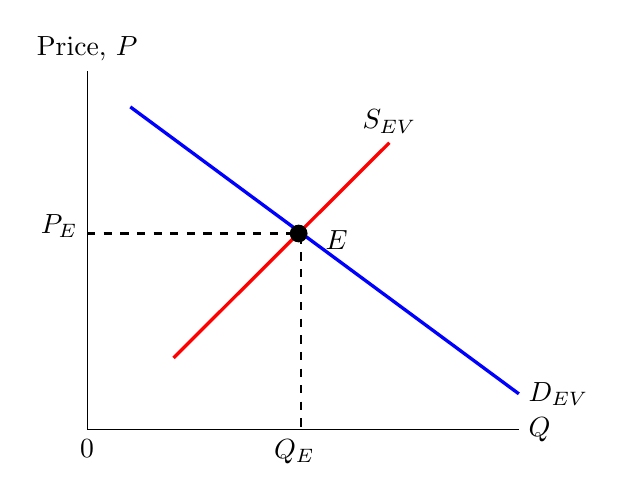
\begin{tikzpicture}
				\begin{axis}[
					scale = .8,
					xmin = 0, xmax = 10,
					ymin = 0, ymax = 10,
					axis lines* = left,
					xtick = {0}, ytick = \empty,
					axis on top,
					clip = false,
					]
					% Colouring areas
					%\fill[orange, opacity = 0.1] (0, 7.67) -- (0, 3.67) -- (5.5, 3.67) -- (5.5, 7.67);
					%\fill[green, opacity = 0.1] (5.5, 0) -- (5.5, 3.67) -- (7, 3.67) -- (7, 0);
					
					% Supply and demand curves
					\addplot[color = blue, very thick] coordinates {(1,9) (10,1)};
					\addplot[color = red, very thick] coordinates {(2,2) (7,8)};
					%\addplot[color = red, opacity = 0.5, very thick] coordinates {(6,1) (9,9)};
					
					% Dashed lines
					\addplot[color = black, dashed, thick] coordinates {(0, 5.47) (4.95, 5.47) (4.95, 0)};
					%\addplot[color = black, dashed, thick] coordinates {(0, 3.67) (7, 3.67) (7, 0)};
					
					% Coordinate points
					\addplot[color = black, mark = *, only marks, mark size = 3pt] coordinates {(4.9, 5.47)};
					
					% Labels
					\node [right] at (current axis.right of origin){$Q$};
					\node [above] at (current axis.above origin) {Price, $P$};
					\node [right] at (5.3, 5.3) {$E$};
					%\node [right] at (7, 3.67) {$E^\prime$};
					\node [right] at (10, 1) {$D_{EV}$};
					\node [above] at (7, 8) {$S_{EV}$};
					%\node [right] at (9, 9) {$S^\prime$};
					\node [left] at (0, 5.67) {$P_E$};
					%\node [left] at (0, 3.67) {$P^\prime$};
					\node [below] at (4.8, 0) {$Q_E$};
					%\node [below] at (7, 0) {$Q^\prime$};
					
					
					% Arrows
					%\draw[-{Triangle[length = 4mm, width = 2mm]}, red, opacity = 0.3] (6.3, 8.5) to (8.3, 8.5);
					%\draw[-Triangle] (5, 11) to [out = 180, in = 90] (2, 6);
					%\draw[-Triangle] (10, -1.5) to [out = 90, in = 0] (6.5, 0.7);
					
				\end{axis}
			\end{tikzpicture}
		\end{center}
		
		\begin{center}
			\emph{Figure 1}\\
		\end{center}
		\tab Tax credit subsidies work by lowering the per-unit cost of a good. When California introduced the \$7,500 tax credit subsidies in 2008, this effectively lowered the price of electric vehicles. This can be seen as a rightward shift of the supply curve, as seen in Figure 2.
		\\
		\\
		\\
		\begin{center}
			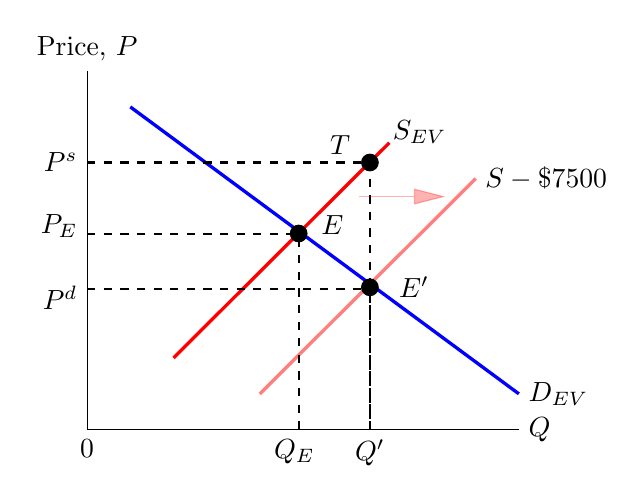
\begin{tikzpicture}
				\begin{axis}[
					scale = .8,
					xmin = 0, xmax = 10,
					ymin = 0, ymax = 10,
					axis lines* = left,
					xtick = {0}, ytick = \empty,
					axis on top,
					clip = false,
					]
					% Colouring areas
					%\fill[orange, opacity = 0.1] (0, 7.67) -- (0, 3.67) -- (5.5, 3.67) -- (5.5, 7.67);
					%\fill[green, opacity = 0.1] (5.5, 0) -- (5.5, 3.67) -- (7, 3.67) -- (7, 0);
					
					% Supply and demand curves
					\addplot[color = blue, very thick] coordinates {(1,9) (10,1)};
					\addplot[color = red, very thick] coordinates {(2,2) (7,8)};
					\addplot[color = red, opacity = 0.5, very thick] coordinates {(4,1) (9,7)};
					
					% Dashed lines
					\addplot[color = black, dashed, thick] coordinates {(0, 5.45) (4.9, 5.45) (4.9, 0)};
					\addplot[color = black, dashed, thick] coordinates {(0, 3.93) (6.55, 3.93) (6.55, 0)};
					\addplot[color = black, dashed, thick] coordinates {(0, 7.45) (6.55, 7.45) (6.55, 0)};
					
					% Coordinate points
					\addplot[color = black, mark = *, only marks, mark size = 3pt] coordinates {(4.9, 5.47) (6.55, 3.97) (6.55, 7.45)};
					
					% Labels
					\node [right] at (current axis.right of origin){$Q$};
					\node [above] at (current axis.above origin) {Price, $P$};
					\node [right] at (5.2, 5.7) {$E$};
					\node [right] at (7, 3.97) {$E^\prime$};
					\node [right] at (10, 1) {$D_{EV}$};
					\node [above] at (7.7, 7.7) {$S_{EV}$};
					\node [right] at (9, 7) {$S-\$7500$};
					\node [left] at (0, 5.67) {$P_{E}$};
					\node [left] at (0, 3.67) {$P^{d}$};
					\node [below] at (4.8, 0) {$Q_{E}$};
					\node [below] at (6.55, 0) {$Q^\prime$};
					\node [left] at (0, 7.45) {$P^{s}$};
					\node [right] at (5.4, 7.95) {$T$};
					
					
					% Arrows
					\draw[-{Triangle[length = 4mm, width = 2mm]}, red, opacity = 0.3] (6.3, 6.5) to (8.3, 6.5);
					%\draw[-Triangle] (5, 11) to [out = 180, in = 90] (2, 6);
					%\draw[-Triangle] (10, -1.5) to [out = 90, in = 0] (6.5, 0.7);
					
				\end{axis}
			\end{tikzpicture}
		\end{center}
		\begin{center}
			\emph{Figure 2}\\
		\end{center}
		There are several attributes of Figure 2 to note. As the subsidy is introduced, the equilibrium price falls from $P_{E}$ to $P^{d}$. Note that the price does not fall by the full \$7,500. The vertical distance from $P_{s}$ to $P^{d}$ represents the entirety of the tax subsidy. \\
		\tab Furthermore, the quantity demanded in the market for electric vehicles increases from $Q_{E}$ to $Q^{\prime}$. As the price of electric vehicles falls from the subsidy introduction, more electric vehicles are bought by consumers, evident in both Figure 2 and Figure 5. This underscores both the theory of demand and using subsidies to incentivize behavior.\\
		\tab The \$7,500 subsidy makes EV's less expensive, holding all other income constant; consumers who otherwise would buy an ICE vehicle may be incentivized to buy an EV.  Figure 5 illustrates an outward pivot of the budget line as more EV's are purchased due to the lower cost. \\
		\newpage
		\begin{center}
			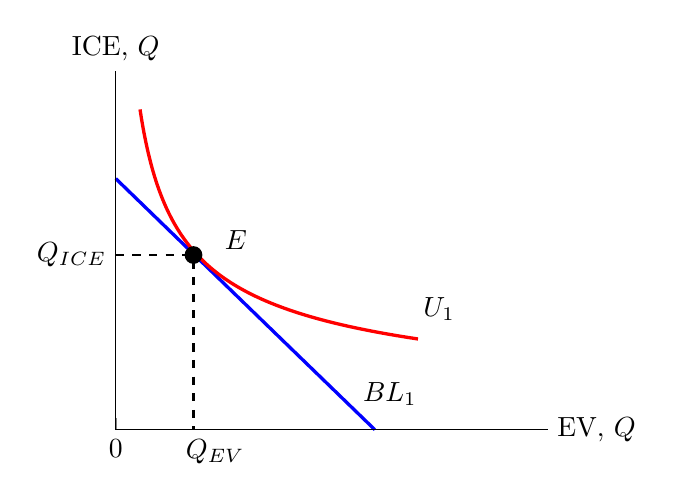
\begin{tikzpicture}
				\begin{axis}[
					scale = .8,
					xmin = 0, xmax = 10,
					ymin = 0, ymax = 10,
					axis lines* = left,
					xtick = {0}, ytick = \empty,
					axis on top,
					clip = false,
					]
					% Colouring areas
					%\fill[orange, opacity = 0.1] (0, 7.67) -- (0, 3.67) -- (5.5, 3.67) -- (5.5, 7.67);
					%\fill[green, opacity = 0.1] (5.5, 0) -- (5.5, 3.67) -- (7, 3.67) -- (7, 0);
					
					% Supply and demand curves
					\addplot[color = blue, very thick] coordinates {(0,7) (6,0)};
					\addplot [domain = 0:7, restrict y to domain = 0:9, samples = 400, color = red, very thick] {8.7*(1/(1.3*x^.5))};
					%\addplot[color = red, very thick] coordinates {(2,2) (7,8)};
					%\addplot[color = red, opacity = 0.5, very thick] coordinates {(6,1) (9,9)};
					
					
					
					% Dashed lines
					\addplot[color = black, dashed, thick] coordinates {(0, 4.87) (1.8, 4.87) (1.8, 0)};
					%\addplot[color = black, dashed, thick] coordinates {(0, 3.67) (7, 3.67) (7, 0)};
					
					% Coordinate points
					\addplot[color = black, mark = *, only marks, mark size = 3pt] coordinates {(1.8, 4.87)};
					
					% Labels
					\node [right] at (current axis.right of origin){EV, $Q$};
					\node [above] at (current axis.above origin) {ICE, $Q$};
					\node [right] at (2.3, 5.3) {$E$};
					\node [right] at (6.9, 3.37) {$U_{1}$};
					\node [right] at (5.5, 1) {$BL_{1}$};
					%\node [above] at (7, 8) {$S_{EV}$};
					%\node [right] at (9, 9) {$S^\prime$};
					\node [left] at (0, 4.87) {$Q_{ICE}$};
					%\node [left] at (0, 3.67) {$P^\prime$};
					\node [below] at (2.3, 0) {$Q_{EV}$};
					%\node [below] at (7, 0) {$Q^\prime$};
					
					
					% Arrows
					%\draw[-{Triangle[length = 4mm, width = 2mm]}, red, opacity = 0.3] (6.3, 8.5) to (8.3, 8.5);
					%\draw[-Triangle] (5, 11) to [out = 180, in = 90] (2, 6);
					%\draw[-Triangle] (10, -1.5) to [out = 90, in = 0] (6.5, 0.7);
					
				\end{axis}
			\end{tikzpicture}
		\end{center}
		\begin{center}
			\emph{Figure 3}\\
		\end{center}
		\tab The subsidy decreases the price of EV's, therefore shifting out the budget line for electric vehicles as shown in Figure 4. Figure 3 illustrates the budget line for EV's before the subsidy took effect. The quantity of EV's increases from $Q_{EV}$ to $Q_{EV}^{\prime}$. The increased demand of EV's causes the quantity demanded of ICE vehicles to decrease, as shown in Figure 5. 
		\begin{center}
			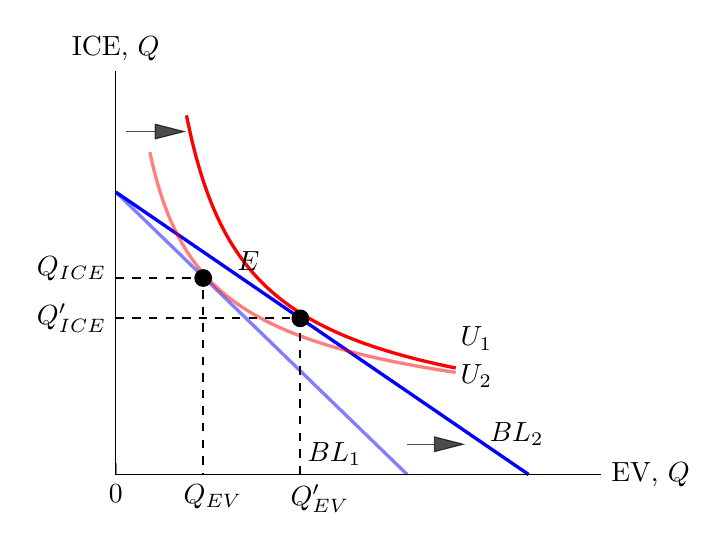
\begin{tikzpicture}
				\begin{axis}[
					scale = .9,
					xmin = 0, xmax = 10,
					ymin = 0, ymax = 10,
					axis lines* = left,
					xtick = {0}, ytick = \empty,
					axis on top,
					clip = false,
					]
					% Colouring areas
					%\fill[orange, opacity = 0.1] (0, 7.67) -- (0, 3.67) -- (5.5, 3.67) -- (5.5, 7.67);
					%\fill[green, opacity = 0.1] (5.5, 0) -- (5.5, 3.67) -- (7, 3.67) -- (7, 0);
					
					% Supply and demand curves
					\addplot[color = blue, opacity = 0.5, very thick] coordinates {(0,7) (6,0)};
					\addplot[color = blue, very thick] coordinates {(0,7) (8.5,0)};
					\addplot [domain = 0:7, restrict y to domain = 0:8, samples = 400, color = red, opacity = 0.5, very thick] {8.7*(1/(1.3*x^.5))};
					\addplot [domain = 0:7, restrict y to domain = 0:9, samples = 400, color = red, very thick] {27*(1/(5*x^.5-3))};
					%\addplot[color = red, very thick] coordinates {(2,2) (7,8)};
					%\addplot[color = red, opacity = 0.5, very thick] coordinates {(6,1) (9,9)};
					
					
					
					% Dashed lines
					\addplot[color = black, dashed, thick] coordinates {(0, 4.87) (1.8, 4.87) (1.8, 0)};
					\addplot[color = black, dashed, thick] coordinates {(0, 3.87) (3.8, 3.87) (3.8, 0)};
					
					% Coordinate points
					\addplot[color = black, mark = *, only marks, mark size = 3pt] coordinates {(1.8, 4.87)};
					\addplot[color = black, mark = *, only marks, mark size = 3pt] coordinates {(3.8, 3.87)};
					
					% Labels
					\node [right] at (current axis.right of origin){EV, $Q$};
					\node [above] at (current axis.above origin) {ICE, $Q$};
					\node [right] at (2.3, 5.3) {$E$};
					\node [right] at (6.9, 3.37) {$U_{1}$};
					\node [right] at (6.9, 2.45) {$U_{2}$};
					\node [right] at (3.75, .5) {$BL_{1}$};
					\node [right] at (7.5, 1) {$BL_{2}$};
					%\node [above] at (7, 8) {$S_{EV}$};
					%\node [right] at (9, 9) {$S^\prime$};
					\node [left] at (0, 5.1) {$Q_{ICE}$};
					\node [left] at (0, 3.87) {$Q_{ICE}^{\prime}$};
					%\node [left] at (0, 3.67) {$P^\prime$};
					\node [below] at (2, 0) {$Q_{EV}$};
					\node [below] at (4.2, 0) {$Q_{EV}^{\prime}$};
					%\node [below] at (7, 0) {$Q^\prime$};
					
					
					% Arrows
					% Arrows
					\draw[-{Triangle[length = 4mm, width = 2mm]}, black, opacity = 0.7] (0.2, 8.5) to (1.45, 8.5);
					\draw[-{Triangle[length = 4mm, width = 2mm]}, black, opacity = 0.7] (6, .75) to (7.2, .75);
					%\draw[-Triangle] (5, 11) to [out = 180, in = 90] (2, 6);
					%\draw[-Triangle] (10, -1.5) to [out = 90, in = 0] (6.5, 0.7);
					
				\end{axis}
			\end{tikzpicture}
		\end{center}
		\begin{center}
			\emph{Figure 4}\\
		\end{center}
		\\
		.
		\bigskip
		\bigskip
		\bigskip
		\begin{center}
			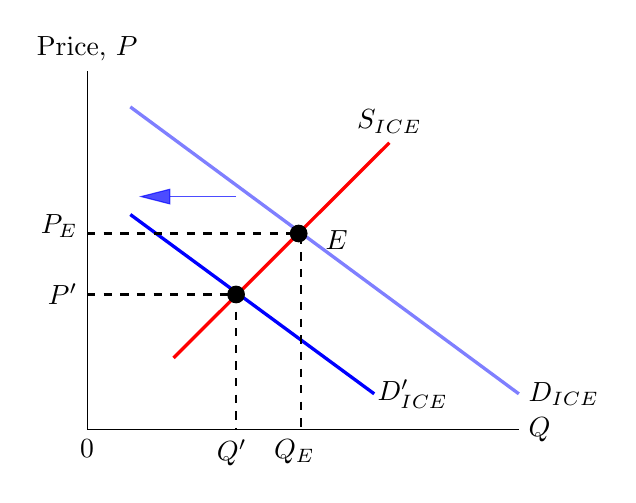
\begin{tikzpicture}
				\begin{axis}[
					scale = .8,
					xmin = 0, xmax = 10,
					ymin = 0, ymax = 10,
					axis lines* = left,
					xtick = {0}, ytick = \empty,
					axis on top,
					clip = false,
					]
					% Colouring areas
					%\fill[orange, opacity = 0.1] (0, 7.67) -- (0, 3.67) -- (5.5, 3.67) -- (5.5, 7.67);
					%\fill[green, opacity = 0.1] (5.5, 0) -- (5.5, 3.67) -- (7, 3.67) -- (7, 0);
					
					% Supply and demand curves
					\addplot[color = blue, opacity = .5, very thick] coordinates {(1,9) (10,1)};
					\addplot[color = blue, very thick] coordinates {(1,6) (6.65,1)};
					\addplot[color = red, very thick] coordinates {(2,2) (7,8)};
					%\addplot[color = red, opacity = 0.5, very thick] coordinates {(6,1) (9,9)};
					
					% Dashed lines
					\addplot[color = black, dashed, thick] coordinates {(0, 5.47) (4.95, 5.47) (4.95, 0)};
					\addplot[color = black, dashed, thick] coordinates {(0, 3.77) (3.45, 3.77) (3.45, 0)};
					
					% Coordinate points
					\addplot[color = black, mark = *, only marks, mark size = 3pt] coordinates {(4.9, 5.47)};
					\addplot[color = black, mark = *, only marks, mark size = 3pt] coordinates {(3.45, 3.77)};
					
					% Labels
					\node [right] at (current axis.right of origin){$Q$};
					\node [above] at (current axis.above origin) {Price, $P$};
					\node [right] at (5.3, 5.3) {$E$};
					%\node [right] at (7, 3.67) {$E^\prime$};
					\node [right] at (10, 1) {$D_{ICE}$};
					\node [right] at (6.5, 1) {$D_{ICE}^{\prime}$};
					\node [above] at (7, 8) {$S_{ICE}$};
					%\node [right] at (9, 9) {$S^\prime$};
					\node [left] at (0, 5.67) {$P_E$};
					\node [left] at (0, 3.77) {$P^\prime$};
					\node [below] at (4.8, 0) {$Q_E$};
					\node [below] at (3.35, 0) {$Q^{\prime}$};
					%\node [below] at (7, 0) {$Q^\prime$};
					
					
					% Arrows
					\draw[-{Triangle[length = 4mm, width = 2mm]}, blue, opacity = 0.7] (3.45, 6.5) to (1.2, 6.5);
					%\draw[-Triangle] (5, 11) to [out = 180, in = 90] (2, 6);
					%\draw[-Triangle] (10, -1.5) to [out = 90, in = 0] (6.5, 0.7);
					
				\end{axis}
			\end{tikzpicture}
		\end{center}
		\begin{center}
			\emph{Figure 5}\\
		\end{center}
		\tab As consumer demand for EVs increases, either the demand for internal combustion engine (ICE) vehicles will decline (at least relative to levels sans the subsidy), or, consumers opt to buy an EV when they normally would not have. Some consumers may choose to buy and then use their EVs primarily for shorter trips while still owning an ICE vehicle. Both circumstances may lead to a reduction in nitrogen oxides ($\text{NO}_\text{x}$) concentrations.\\ 
		\tab Figure 7 shows that after the first EV subsidy was introduced in California, monthly Battery Electric Vehicle (BEV) subsidy applications gradually increased over time, reaching 1,000 per month in 2013 and 3,000 per month in 2015. Additionally, Figure 6 illustrates the changes in ZIP code-level BEV concentrations between 2010 and 2016. Though EV adoption expanded greatly during this time frame, we see greater concentrations of EVs in urban centers, including San Diego, Los Angeles, and the San Francisco bay area.\\
		\tab While this paper does not seek to establish a causal relationship between subsidy implementation and EV adoption, Figures 8 and 9 indicate a clear correlation between the two, which is instrumental in determining the pre and post dimensions of the DiD analysis. Using ZIP code-level EV adoption data, this paper examines how subsidy implementation influenced air quality throughout the state. By analyzing changes in nitrogen dioxide concentrations, we aim to assess whether increased EV adoption contributed to improved air quality in California.
		
	\end{multicols}
	
	
	\begin{Figure}
		\centering
		\includegraphics[width=\linewidth]{Model Free Evidence/bev_2010_vs_2016.png}
		
		%\captionof{figure}{my caption of the figure}
	\end{Figure}
	\begin{center}
		\emph{Figure 6}\\
	\end{center}
	
	
	
	
	\setcounter{figure}{6}
	\begin{center}
		\includegraphics[width=\linewidth]{Model Free Evidence/ev_subsidies_over_time_bw.png}
		\captionof{figure}{\footnotesize  BEV: Battery Electric; FCEV: Fuel Cell Electric; PHEV: Plug-in Hybrid Electric}
		\label{fig:ev_subs_per_month}
	\end{center}
	\begin{center}
		\emph{Figure 7}\\
	\end{center}
	\begin{multicols}{2}
		
		\section*{Data}
		\addcontentsline{toc}{section}{Data}
		Data are collected from a multitude of sources, through both APIs, direct downloads from resources published by state of California, the US Environmental Protection Agency (EPA), and the United States Department of Agriculture (USDA). This paper creates a panel dataset that includes the following variables and their respective granularity. \\
		\tab In this paper, air quality (or pollution) is measured by the concentrations of Nitrogen Dioxide $\text{NO}_\text{2}$ in the atmosphere. $\text{NO}_\text{2}$ (parameter code 42602) is measured in parts-per-billion (ppb) and obtained through the EPA via an API. Measurements are made once per day for a duration of 60 minutes. California has 129 sites throughout the state, resulting in approximately 329,000 observations (129 sites $\times$ 7 years $\times$ 365 days). The $\text{NO}_\text{2}$ dataset also includes the county, site address, latitude and longitude, and CBSA code. Figure 8 depicts a map of the 129 air quality measurement sites. Figure 20 illustrates trends in $NO_2$ between 2010 and 2017.\\
		\tab  Agriculture data used in this paper come from two different sources, the United States Department of Agriculture (USDA) and the California Department of Food and Agriculture. The first dataset, from the USDA, provides a county-level break down of agriculture acreage in California based on the following categories, denoted in acres: Fertilizer (Total), Fertilizer (Organic), Fertilizer (Manure), Chemical Insecticide, Chemical Herbicide, Chemical Fungicide, and Insecticide (Nematicides). These data range from 2004 to 2022, with data points occurring every five years. The Fertilizer (Total) acreage in 2012 is illustrated in Figure 10.\\
		\tab The second dataset, from the California Department of Food and Agriculture, provides the tonnage of different types of fertilizers at the county-level. Out of the thirty fertilizers collected in the dataset, this paper focuses on the five most Nitrogen dense, including Anhydrous Ammonia (82\% Nitrogen), Urea (46\% Nitrogen), Ammonium Nitrate (33-34\% Nitrogen), Nitrate Solution (32-34\% Nitrogen), and Urea Solution (30\% Nitrogen)\footnote{International Fertilizer Association (IFA) https://www.fertilizer.org}. As we are interested in controlling for the $\text{NO}_\text{x}$ released from fertilizers, it is important to add fertilizer tonnage as control variables. The concentrations of the top 5 most nitrogen-dense fertilizers throughout the state can be visualized in Figures 11-15. \\
		\tab Data on vehicle population (number of cars on the road) come from the California Energy Commission. The number of cars on the road are reported yearly at both the county and ZIP code-level, broken down by vehicle type, which include Battery Electric (BEV), Gasoline, Gasoline Hybrid, Diesel, Plug-in-Hybrid, Flex-Fuel, Natural Gas, and Propane. Vehicle population is updated annually, each April, to reflect the number of vehicles “on the road” during the previous calendar year. Vehicle population counts vehicles whose registration is either current or less than 35 days expired. Sales are higher than population because of vehicle retirements, accidents, owners moving out of state, or other reasons (California Energy Commission). Total vehicle population by county is illustrated in Figure 9.\\
		\tab New zero emission vehicle (ZEV) sales are reported by the California Energy Commission. New ZEV sales (a subset of which are EVs) are recorded at the county and ZIP code level, and dates range from 1998 to 2024. ZEV include Electric, Hydrogen, and Plug-in-Hybrid vehicles; this paper focuses on the EV subset. Zero Emission Vehicles (ZEV) sales are updated on a quarterly basis by examining the DMV Vehicle Registration database for vehicles which show no evidence of transfer of ownership, and were purchased within the specified time frame. To account for vehicles which may have been brought in from outside California, only those vehicles with a low odometer reading are treated as new sales (California Energy Commission). Figure 16 depicts the change in new EV sales between 2010 and 2016. \\
		\tab EV subsidy data are also reported by the California Energy Commission. Subsidy applications per day are recorded by county and ZIP code, and also include the rebate amount for each individual application. The dataset also denotes whether the application was flagged as a low-income EV subsidy. Daily data range from March 2010 through April 2024. Figure 7 (above) illustrates the trend in EV applications over time, aggregated at the monthly level. Figure 17 depicts the concentration of low-income rebates in four major cities throughout California.  \\
		\tab County level population and income per capita data are accessed through an API offered by the Bureau of Economic analysis (BEA) and range from 2004 to 2024. Data are filtered to fit the scope of this paper. Figures 18 and 19 illustrate county level population and income per capita, respectively, in 2010.  \\ 
		
		
	\end{multicols}
	
	\begin{multicols}{2}
		
		
		\begin{Figure}
			\centering
			\includegraphics[width=\linewidth]{Model Free Evidence/air_quality_sites.png}
			
			%\captionof{figure}{my caption of the figure}
		\end{Figure}
		\begin{center}
			\emph{Figure 8}\\
		\end{center}
		
		
		
		\begin{Figure}
			\centering
			\includegraphics[width=\linewidth]{Model Free Evidence/all_vehicles_2010.png}
			
			%\captionof{figure}{my caption of the figure}
		\end{Figure}
		\begin{center}
			\emph{Figure 9}\\
		\end{center}
		
		
		
		
		\begin{Figure}
			\centering
			\includegraphics[width=\linewidth]{Model Free Evidence/fertilizer_usage_2012.png}
			
			%\captionof{figure}{my caption of the figure}
		\end{Figure}
		\begin{center}
			\emph{Figure 10}\\
		\end{center}
		
		
		
		% 
		
		\begin{Figure}
			\centering
			\includegraphics[width=\linewidth]{Model Free Evidence/anhydrous_ammonia.png}
			
			%\captionof{figure}{my caption of the figure}
		\end{Figure}
		\begin{center}
			\emph{Figure 11}\\
		\end{center}
		
		% 
		
		\begin{Figure}
			\centering
			\includegraphics[width=\linewidth]{Model Free Evidence/urea.png}
			
			%\captionof{figure}{my caption of the figure}
		\end{Figure}
		\begin{center}
			\emph{Figure 12}\\
		\end{center}
		
		
		% 
		
		\begin{Figure}
			\centering
			\includegraphics[width=\linewidth]{Model Free Evidence/ammonium nitrate.png}
			
			%\captionof{figure}{my caption of the figure}
		\end{Figure}
		\begin{center}
			\emph{Figure 13}\\
		\end{center}
		
		
		% 
		
		\begin{Figure}
			\centering
			\includegraphics[width=\linewidth]{Model Free Evidence/nitrate solution.png}
			
			%\captionof{figure}{my caption of the figure}
		\end{Figure}
		\begin{center}
			\emph{Figure 14}\\
		\end{center}
		
		
		
		\begin{Figure}
			\centering
			\includegraphics[width=\linewidth]{Model Free Evidence/urea solution.png}
			
			%\captionof{figure}{my caption of the figure}
		\end{Figure}
		\begin{center}
			\emph{Figure 15}\\
		\end{center}
		
		
	\end{multicols}
	
	\newpage
	
	\begin{Figure}
		\centering
		\includegraphics[width=\linewidth]{Model Free Evidence/new ev sales.png}
		
		%\captionof{figure}{my caption of the figure}
	\end{Figure}
	\begin{center}
		\emph{Figure 16}\\
	\end{center}
	
	
	\begin{Figure}
		\centering
		\includegraphics[width=\linewidth]{Model Free Evidence/low_income_rebates_by_four_cities.png}
		
		%\captionof{figure}{my caption of the figure}
	\end{Figure}
	\begin{center}
		\emph{Figure 17}\\
	\end{center}
	\newpage
	\begin{multicols}{2}
		% 
		\begin{Figure}
			\centering
			\includegraphics[width=\linewidth]{Model Free Evidence/ca_pop.png}
			
			%\captionof{figure}{my caption of the figure}
		\end{Figure}
		\begin{center}
			\emph{Figure 18}\\
		\end{center}
		
		\begin{Figure}
			\centering
			\includegraphics[width=\linewidth]{Model Free Evidence/income_per_capita.png}
			
			%\captionof{figure}{my caption of the figure}
		\end{Figure}
		\begin{center}
			\emph{Figure 19}\\
		\end{center}
		
	\end{multicols}
	\begin{Figure}
		\centering
		\includegraphics[width=\linewidth]{Model Free Evidence/monthly_no2.png}
		
		%\captionof{figure}{my caption of the figure}
	\end{Figure}
	\begin{center}
		\emph{Figure 20}\\
	\end{center}
	
	
	
	\clearpage
	\subsection*{Summary Statistics}
	\addcontentsline{toc}{section}{Summary Statistics}
	
	\begin{table}[h]
		\centering
		\begin{minipage}{0.48\textwidth}
			\centering
			\caption{NO$_2$ Summary Statistics (ppb)}
			\label{tab:no2_summary}
			\begin{tabular}{l c c c c}
				\toprule
				Year & Mean & Std. Dev. & Min & Max \\
				\midrule
				2010 & 11.00 & 8.44 & 0.00 & 57.30 \\
				2011 & 11.00 & 8.47 & 0.00 & 62.50 \\
				2012 & 10.40 & 7.92 & -1.80 & 66.70 \\
				2013 & 10.50 & 8.24 & -1.05 & 57.80 \\
				2014 & 9.96 & 8.21 & -2.38 & 63.70 \\
				2015 & 9.85 & 8.26 & -2.50 & 60.20 \\
				\bottomrule
			\end{tabular}
		\end{minipage}
		\hfill
		\begin{minipage}{0.48\textwidth}
			\centering
			\caption{Population Summary Statistics (County-Year Level)}
			\label{tab:population_summary}
			\begin{tabular}{l c c c c}
				\toprule
				Year & Mean & Std. Dev. & Min & Max \\
				\midrule
				2010 & 1,034,977 & 1,724,152 & 94,814 & 9,822,677 \\
				2011 & 1,067,306 & 1,756,433 & 94,827 & 9,878,903 \\
				2012 & 1,106,357 & 1,787,586 & 94,803 & 9,940,845 \\
				2013 & 1,116,027 & 1,799,545 & 95,399 & 10,000,924 \\
				2014 & 1,126,289 & 1,810,006 & 95,959 & 10,051,511 \\
				2015 & 1,136,076 & 1,819,964 & 96,764 & 10,099,677 \\
				\bottomrule
			\end{tabular}
		\end{minipage}
	\end{table}
	
	\begin{table}[h]
		\centering
		\begin{minipage}{0.48\textwidth}
			\centering
			\caption{Income Per Capita Summary (County-Year Level)}
			\label{tab:income_summary}
			\begin{tabular}{l c c c c}
				\toprule
				Year & Mean & Std. Dev. & Min & Max \\
				\midrule
				2010 & 42,291 & 13,680 & 26,345 & 83,247 \\
				2011 & 44,234 & 15,023 & 29,308 & 89,206 \\
				2012 & 46,079 & 17,188 & 28,626 & 94,993 \\
				2013 & 46,755 & 16,882 & 29,642 & 95,473 \\
				2014 & 49,340 & 18,311 & 32,810 & 102,032 \\
				2015 & 52,386 & 20,221 & 32,733 & 109,274 \\
				\bottomrule
			\end{tabular}
		\end{minipage}
		\hfill
		\begin{minipage}{0.48\textwidth}
			\centering
			\caption{Total Cars Summary (County-Year Level)}
			\label{tab:total_cars_summary}
			\begin{tabular}{l c c c c}
				\toprule
				Year & Mean & Std. Dev. & Min & Max \\
				\midrule
				2010 & 603,200 & 982,527 & 56,545 & 5,533,454 \\
				2011 & 615,818 & 992,569 & 56,564 & 5,519,793 \\
				2012 & 636,818 & 1,006,949 & 56,495 & 5,535,594 \\
				2013 & 658,738 & 1,038,871 & 58,353 & 5,703,872 \\
				2014 & 676,660 & 1,065,050 & 59,909 & 5,845,470 \\
				2015 & 691,569 & 1,086,548 & 61,199 & 5,962,163 \\
				\bottomrule
			\end{tabular}
		\end{minipage}
	\end{table}
	
	
	\clearpage
	
	\begin{multicols}{2}
		Table 1 through Table 4 show select summary statistics. $NO_2$ concentrations exhibit a gradual decline from 2010 to 2015, with mean values decreasing from 11.00 ppb to 9.85 ppb. The standard deviation remains relatively stable, suggesting consistent variability in pollution levels across sites. The maximum$NO_2$ values, however, fluctuate, reflecting episodic pollution spikes likely influenced by weather patterns or localized emissions events. County-level population trends indicate steady growth, with the mean increasing from $1,034,977$ in 2010 to $1,136,076$ in 2015. The large standard deviation suggests substantial variation across counties, reflecting the presence of both highly urbanized and sparsely populated regions.\\ 
		
		\section*{Methodology}
		\addcontentsline{toc}{section}{Methodology}
		
		This section outlines the methodology used in assessing the relationship between EV subsidy implementation and reduced air pollution.\\
		\tab The classification of high EV adoption ZIP codes is a crucial step in identifying the potential impact of electric vehicle (EV) adoption on air quality. This study defines high EV adoption ZIP codes based on the relationship between the growth in EV subsidy applications and the number of new EVs on the road within a given ZIP code. Specifically, a ZIP code is considered to have high EV adoption if its growth in EV subsidies surpasses a threshold relative to its baseline EV stock. The growth rate of EV subsidy applications and the growth in the number of EVs is calculated between 2011 and 2012, using the following formula:
		
		\begin{align}
			G_{\text{zip}} = \frac{EV_{\text{zip},2012} - EV_{\text{zip},2011}}{EV_{\text{zip},2011} + 1}
		\end{align}
		
		where:
		\begin{itemize}
			\item \( G_{\text{zip}} \) represents the EV growth rate in ZIP code \( \text{zip} \),
			\item \( EV_{\text{zip},2012} \) and \( EV_{\text{zip},2011} \) represent the number of registered EVs in ZIP \( \text{zip} \) in 2012 and 2011, respectively,
			\item The +1 in the denominator prevents division by zero in ZIP codes with no EVs in 2011.
		\end{itemize}
		
		A ZIP code is considered high EV adoption if \( G_{\text{zip}} \) exceeds a predetermined threshold. This paper uses a 25\% increase in EV subsidy applications between 2011 and 2012 as the initial threshold; other values are also tested as part of the robustness checks, including 15\%, 35\%, and 50\%. \\
		\tab Once high EV adoption ZIP codes are identified, we relate each air quality monitoring site to the nearest ZIP code using the Haversine formula, which calculates the great-circle distance between two latitude-longitude pairs. Using the \emph{maps} functionality in R, we relate each ZIP code to a set of boundary latitude and longitude points. The Haversine function is given by:
	\end{multicols}
	\begin{align}
		d = 2r \cdot \arcsin \left( \sqrt{\sin^2\left(\frac{\Delta \varphi}{2}\right) + \cos(\varphi_1) \cdot \cos(\varphi_2) \cdot \sin^2\left(\frac{\Delta \lambda}{2}\right)} \right)
	\end{align}
	
	where:
	\begin{itemize}
		\item \( d \) is the distance between two points (ZIP centroid and air quality site),
		\item \( r \) is the Earth’s radius (\(\approx 6371\) km),
		\item \( \varphi_1, \varphi_2 \) are the **latitudes of the two points** in radians,
		\item \( \lambda_1, \lambda_2 \) are the longitudes of the two points in radians,
		\item \( \Delta \varphi = \varphi_2 - \varphi_1 \) and \( \Delta \lambda = \lambda_2 - \lambda_1 \).
	\end{itemize}
	\newpage
	
	\begin{multicols}{2}
		
		
		Each air quality site is assigned to the closest ZIP code based on the minimum Haversine distance. If the nearest ZIP code is classified as high EV adoption, the air quality site is also considered to be in an area of high EV adoption. Conversely, if the nearest ZIP code does not meet the high EV adoption threshold, the air quality site is considered in a low EV adoption area.
		
		Finally, air quality sites are categorized into treatment and control groups based on the classification of their associated ZIP codes:
		\begin{itemize}
			\item Treatment: Air quality sites located in ZIP codes with high EV adoption.
			\item Control: Air quality sites located in ZIP codes with low or no EV adoption.
		\end{itemize}
		
		This paper focuses especially on determining EV adoption rates based on the use of the subsidy, and not only by EVs that may have already been purchased but not through the subsidy program. As stated above, there are three measurements of the Electric Vehicle population that may be used: cars on the road, EV subsidy applications, and new EV sales. This analysis is careful to only consider new EV sales and subsidy applications when defining ZIP codes of high EV adoption. This technique allows any changes in air pollution to have a more robust connection to the EV subsidy mechanism, controlling for other factors.\\
		\tab By leveraging geospatial matching techniques and subsidy growth measures, this study establishes a framework to analyze the impact of EV adoption on air quality with localized precision. The spatial treatment assignment ensures that any observed changes in pollution levels can be more accurately attributed to EV adoption trends rather than external influences.\\
		\tab Figure 21 below illustrates the relationship between the county, ZIP codes, and air quality sites. In this example, ZIP code 2 has a rate of EV adoption that exceeds 25\%, while ZIP code 1 does not meet the 25\% threshold,  as determined by Equation 6, and therefore, by comparing spacial coordinates, Air Quality Site A receives treatment status. Meanwhile, Air Quality Site B, which is not close to the high EV adoption ZIP 2, receives control group demarcation.
		
	\end{multicols}
	\setcounter{figure}{20}
	
	\begin{figure}[h]
		\centering
		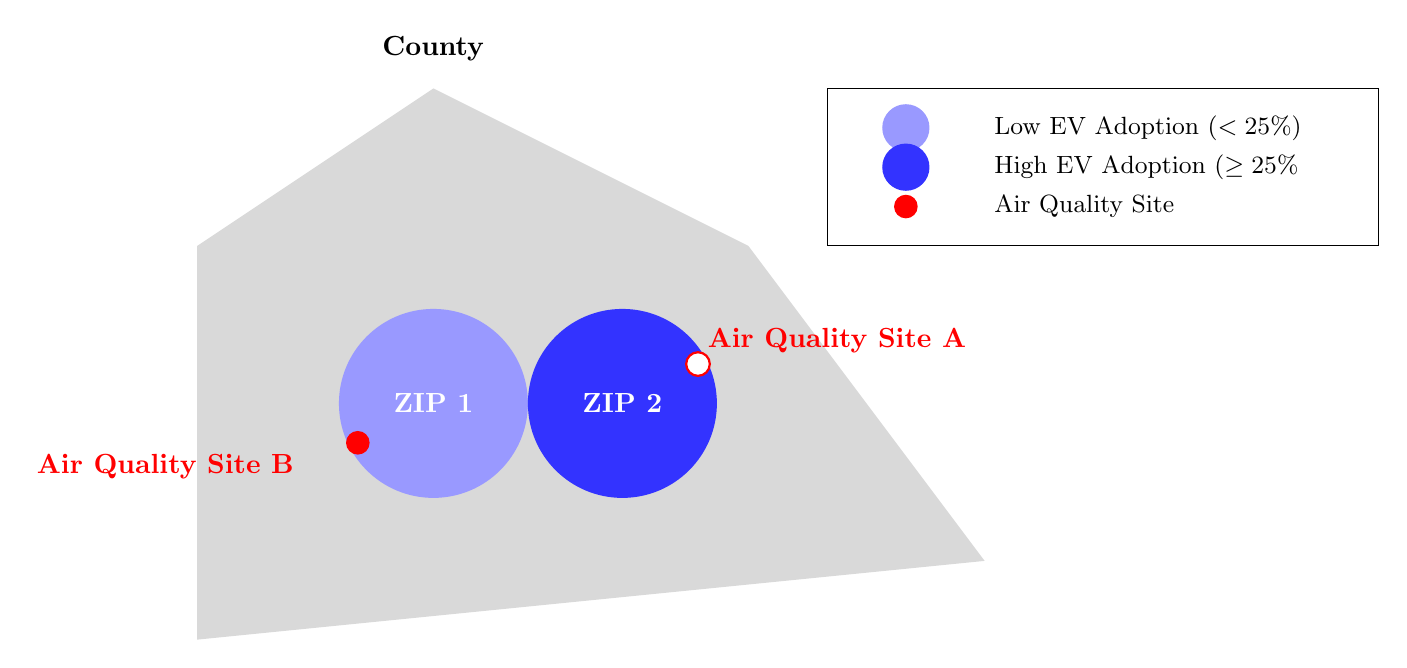
\begin{tikzpicture}
			
			% Draw the county (as an irregular polygon)
			\fill[gray!30] (0,0) -- (10,1) -- (7,5) -- (3,7) -- (0,5) -- cycle;
			
			% Define ZIP code radius
			\def\radius{1.2}
			
			% Draw ZIP Code 1 (lighter blue)
			\fill[blue!40] (3,3) circle (\radius); 
			
			% Draw ZIP Code 2 (darker blue), positioned exactly 2×radius apart to touch tangentially
			\fill[blue!80] (3 + 2*\radius, 3) circle (\radius); 
			
			% Draw the air quality monitoring site (inside the county, near ZIP 2)
			\draw[red, fill=white, thick] (3 + 2.8*\radius, 3.5) circle (0.15);
			\fill[red] (5.4 - 2.8*\radius, 2.5) circle (0.15);
			
			% Labels
			\node at (3,7.5) {\textbf{County}};
			\node[white] at (3,3) {\textbf{ZIP 1}};
			\node[white] at (3 + 2*\radius,3) {\textbf{ZIP 2}};
			\node[red, right] at (3 + 2.8*\radius,3.8) {\textbf{Air Quality Site A}};
			\node[red, right] at (1.2 - 2.8*\radius,2.2) {\textbf{Air Quality Site B}};
			
			% Legend box
			\draw[black] (8,5) rectangle (15,7);
			
			% Legend entries
			\fill[blue!40] (9,6.5) circle (0.3);  % Light blue circle
			\node[right] at (10,6.5) {\small Low EV Adoption $(< 25\%)$};
			
			\fill[blue!80] (9,6) circle (0.3);  % Dark blue circle
			\node[right] at (10,6) {\small High EV Adoption $(\geq 25\%$};
			
			\fill[red] (9,5.5) circle (0.15);  % Red dot for air quality site
			\node[right] at (10,5.5) {\small Air Quality Site};
			
		\end{tikzpicture}
		\caption{Illustration of County, Two Tangential ZIP Codes, and Air Quality Monitoring Sites}
		\label{fig:county_zip_site}
	\end{figure}
	\pagebreak
	\begin{multicols}{2}
		
		\section*{Econometric Specification}
		\addcontentsline{toc}{section}{Econometric Specification}
		
		This paper utilizes a difference in differences approach to estimate the impact of EV subsidy adoption and reduced $\text{NO}_\text{2}$ levels in California.\\
		\tab By leveraging daily air quality monitoring data from 2010 to 2016, this study identifies localized changes in air pollution associated with shifts in EV adoption. The identification strategy exploits variation in EV subsidy applications at the ZIP code level, which are then used to classify air quality monitoring sites as either treatment or control. The 2018 study by Almaraz et al. estimates that 32\% of California's $NO_2$ emissions can be attributed to nitrogen-dense fertilizers, while 35–51\% originate from combustion processes. To isolate the effect of increased EV adoption on $NO_2$ concentrations, this analysis controls for annual variations in fertilizer usage. Specifically, we include controls for total fertilizer application (acres) by county, along with the tonnage (by county) of the five most nitrogen-dense fertilizers to account for their potential contribution on $NO_2$ emissions. \\
		\tab Although the EV subsidy program was introduced around March 2010, Figure 7 suggests that substantial utilization of subsidies did not occur until 2011. Therefore, to incorporate the time dimension into the difference-in-differences framework, we define January 2011 as the cutoff for the pre- and post-treatment periods. Consequently, the post-treatment indicator variable is set to 0 for observations before January 2011 and 1 thereafter. This ensures that any estimated treatment effect captures the impact of increasing EV adoption following the initial phase of subsidy uptake.\\
		\tab The definition of the treatment group is based on the relative increase in EV adoption between 2011 and 2012 rather than the initial policy implementation date. Specifically, a ZIP code is classified as treated if it experienced a 25\% or greater increase in EV adoption between 2011 and 2012, defined by EV subsidy use. Other threshold increase variations are tested in the Robustness Checks section. Once ZIP codes are assigned treatment status, the air quality monitoring site closest to each ZIP centroid inherits the classification, ensuring a geospatially consistent treatment definition. Figure 21 (above) illustrates this relationship. The assignment of treatment and control status is further detailed in the methodology section, where we describe the process of linking EV adoption at the ZIP code level to air quality monitoring sites via spatial proximity.\\
		\tab By structuring the analysis in this manner, the study isolates the localized impact of EV adoption on $NO_2$ concentrations while controlling for broader temporal trends and site-specific characteristics.. The model takes on the functional form of Equation~\ref{eq:DiD_model}.
		
		\begin{align}
			NO_{2_{i,t}} &= \beta_0 + \beta_1 \text{Treatment}_{i} + \beta_2 \text{Post}_{t} + \nonumber \end{align} \begin{align}
			\beta_3 (\text{Treatment}_{i} \times \text{Post}_{t})
			& + \beta_4 X_{i,t} + \nonumber \end{align} \begin{align}
			\gamma_i + \delta_t + \epsilon_{i,t} \label{eq:DiD_model}
		\end{align}
		where:
		\begin{itemize}
			\item \( NO_{2_{i,t}} \) is the nitrogen dioxide concentration in ppb at air quality site \( i \) on day \( t \).
			\item \( \beta_0 \) is the intercept.
			\item \( \text{Treatment}_{i} \) is an indicator variable equal to 1 if air quality site \( i \) is in a high EV adoption area, and 0 otherwise.
			\item \( \text{Post}_{t} \) is an indicator variable equal to 1 if \( t \) is after January 2011, and 0 otherwise.
			\item \( \text{Treatment}_{i} \times \text{Post}_{t} \) is the difference-in-differences interaction term, capturing the effect of increased EV adoption on \(\text{NO}_2\).
			\item \( X_{i,t} \) is a vector of control variables, including total fertilizer usage, nitrogen-dense fertilizers, population, and income per capita.
			\item \( \gamma_i \) represents site fixed effects, controlling for time-invariant differences across monitoring sites.
			\item \( \delta_t \) represents time fixed effects, capturing common time trends.
			\item \( \epsilon_{i,t} \) is the error term.
		\end{itemize} 
		
		The coefficient of interest, $\hat{\beta_3}$, in the difference-in-differences (DiD) framework captures the causal effect of increased EV adoption on nitrogen dioxide ($NO_2$) concentrations. The estimator is constructed by computing the difference in mean $NO_2$ levels before and after treatment for both the treated group ($Treatment_i = 1$) and the control group ($Treatment_i = 0$). This approach isolates the effect of EV adoption by netting out time-invariant differences between treated and control areas as well as common shocks affecting all locations over time. The first bracketed term in Equation \eqref{eq:DiD_estimator} represents the change in $NO_2$ levels in the treated group before and after the treatment period. This captures both the potential impact of EV adoption and any underlying time trends. The second bracketed term reflects the corresponding change in $NO_2$ levels for the control group, which is assumed to evolve similarly to the treatment group in the absence of treatment. By differencing these two terms, the DiD estimator removes time-invariant unobserved heterogeneity and accounts for common macroeconomic and regulatory factors that may influence air quality trends.\\
		\tab A key identifying assumption underlying this specification is the parallel trends assumption, which requires that, absent treatment, the change in $NO_2$ concentrations would have been the same for both treated and control groups. If this assumption holds, then  $\hat{\beta_3}$ provides an unbiased estimate of the impact of EV adoption on $NO_2$ concentrations, net of confounding effects. However, if treated and control groups exhibit diverging pre-trends, the estimated treatment effect may be biased. To assess the validity of this assumption, we conduct robustness checks, including pre-trend analysis, alternative specifications, and placebo tests.\\
		\tab Equation \eqref{eqn:par} represents the parallel trends assumption in a difference-in-differences (DiD) framework, which is a key identification condition for causal inference. The assumption states that, in the absence of treatment (i.e., increased EV adoption), the difference in nitrogen dioxide ($NO_2$) concentrations between treatment and control groups would have remained constant over time.\\
		\tab Mathematically, the left-hand side of the equation captures the pre-treatment difference in $NO_2$ concentrations between treated ($Treatment_i = 1 $) and control ($Treatment_i = 0$) locations before EV adoption significantly increased. The right-hand side represents the post-treatment difference in$NO_2$ levels after the treatment period begins. If the parallel trends assumption holds, any difference observed after treatment can be attributed to the impact of EV adoption rather than to pre-existing differences in pollution trends between the two groups.\\
		\tab This assumption ensures that the control group provides a valid counterfactual for what would have happened to $NO_2$ levels in the treated areas in the absence of high EV adoption. If the parallel trends assumption is violated, the estimated treatment effect may be biased due to systematic differences in the evolution of $NO_2$ levels between the treated and control ZIP codes prior to the treatment period. To assess the validity of this assumption, robustness checks such as pre-trend analysis and placebo tests are conducted.
	\end{multicols}
	\begin{align}
		\hat{\beta}_3 &= \left[ \mathbb{E}( NO_{2_{i,t}} | \text{Treatment}_{i} = 1, \text{Post}_{t} = 1 ) 
		- \mathbb{E}( NO_{2_{i,t}} | \text{Treatment}_{i} = 1, \text{Post}_{t} = 0 ) \right] \nonumber \\
		&\quad - \left[ \mathbb{E}( NO_{2_{i,t}} | \text{Treatment}_{i} = 0, \text{Post}_{t} = 1 ) 
		- \mathbb{E}( NO_{2_{i,t}} | \text{Treatment}_{i} = 0, \text{Post}_{t} = 0 ) \right] \label{eq:DiD_estimator}
	\end{align}
	
	\begin{align}
		\mathbb{E}( NO_{2_{i,t}} | \text{Treatment}_{i} = 1, \text{Post}_{t} = 0 ) - 
		\mathbb{E}( NO_{2_{i,t}} | \text{Treatment}_{i} = 0, \text{Post}_{t} = 0 ) = \nonumber \\
		\mathbb{E}( NO_{2_{i,t}} | \text{Treatment}_{i} = 1, \text{Post}_{t} = 1 ) - 
		\mathbb{E}( NO_{2_{i,t}} | \text{Treatment}_{i} = 0, \text{Post}_{t} = 1 )  \label{eqn:par}
	\end{align}
	
	\begin{multicols}{2}
		
		The parallel trends assumption will be verified in the Robustness Checks section following the results.\\ 
		\tab Including population and income per capita as control variables in the difference-in-differences (DiD) model is essential to account for socioeconomic factors that may independently influence nitrogen dioxide ($NO_2$) concentrations. Population density is directly related to vehicle ownership, traffic congestion, and overall emissions, which can affect ambient air pollution levels. Similarly, income per capita may proxy for differences in consumption patterns, transportation infrastructure, and vehicle preferences, including the adoption of newer, less-polluting vehicles. By including these controls, the model mitigates the risk of omitted variable bias, ensuring that estimated treatment effects more accurately reflect the causal impact of increased electric vehicle (EV) adoption on $NO_2$ concentrations rather than underlying economic differences across locations.\\
		\tab In addition to these controls, the model incorporates county, year, month, and core-based statistical area (CBSA) fixed effects to further address unobserved heterogeneity. Fixed effects control for time-invariant characteristics that differ across geographic units and could confound the estimated treatment effect. County fixed effects capture persistent differences in regulatory policies, industrial composition, and baseline pollution levels that might otherwise bias the results. Year and month fixed effects account for common time trends, such as seasonal fluctuations in emissions and broader macroeconomic conditions. Core-Based Statistical Area refers to a geographic area centered around a significant urban cluster, encompassing surrounding counties where people commute to that urban area. CBSA fixed effects allow for the inclusion of regional economic and demographic patterns that may not be fully captured by county-level variation alone. By absorbing these sources of unobserved heterogeneity, fixed effects ensure that identification comes from within-unit variation over time, strengthening the credibility of the estimated relationship between EV adoption and air quality.\\
		\tab We expect the coefficient on 
		$Treatment_i$ to be positive with a large magnitude, as these counties will most likely have a higher population density, more cars overall, and therefore the base level of $NO_2$ will be higher. The sign on 
		$Post_t$ is ambiguous, as broader economic, regulatory, and environmental trends could either increase or decrease overall $NO_2$ levels between the pre- and post-treatment periods.\\
		\tab Both $population$ and $income\_per\_capita$ are expected to have positive coefficients, as higher population density tends to correlate with greater emissions, and wealthier areas may have more vehicle ownership, potentially increasing baseline emissions.\\
		\tab Similarly, we anticipate a positive coefficient on $total\_fertilizer$ as well as $organic\_fertilizer$, as fertilizers contribute to nitrogen-based emissions which impact air quality. Specifically, $Anhydrous\_Ammonia$, a highly nitrogen-intensive fertilizer, is expected to have a positive coefficient due to its potential contribution to atmospheric nitrogen oxides.\\
		\tab Additionally, we expect $total\_cars$ and $total\_EV\_cars$ to both have positive coefficients. The positive sign on total vehicles is intuitive, as more vehicles contribute to higher emissions, while the positive coefficient on EV cars may reflect correlations with overall vehicle density rather than a direct pollution effect. The net effect of EVs on air quality is captured more directly through the interaction term rather than through aggregate vehicle counts.\\
		\tab Lastly, I expect the coefficient on the DiD Estimator, $\text{Treatment}_{i} \times \text{Post}_{t}$ to be negative, as this paper hypothesizes that in counties with high EV adoption, $NO_2$ levels will be lower after the subsidy begins to take effect. 
		
		\section*{Results}
		\addcontentsline{toc}{section}{Results}
		
		Model 1, shown in Equation \eqref{eqn:model1} and Column 1 of Table 5, provides a baseline estimation of the effect of EV adoption on $NO_2$ concentrations, controlling only for population and income per capita. The coefficient on $Treatment_i$ is positive and significant at the 0.1\% level, suggesting that areas with higher EV adoption tend to have higher baseline $NO_2$ levels. This could be due to higher initial vehicle density in treated ZIP codes. The interaction term on $Treatment_i \times Post_t$ is negative but not statistically significant, suggesting that the policy's impact is not yet well-identified in this specification. The population coefficient is positive and statistically significant, indicating that areas with higher population density tend to have higher pollution levels, which is expected given greater emissions from transportation and industry. Income per capita is negative but not significant, implying that wealthier areas may have slightly lower $NO_2$ levels, potentially due to newer vehicle fleets or better infrastructure.
		\begin{align}
			NO_{2_{i,t}} &= \beta_0 + \beta_1 \text{Treatment}_{i} + \beta_2 \text{Post}_{t} + \nonumber \end{align} \begin{align}
			\beta_3 (\text{Treatment}_{i} \times \text{Post}_{t}) 
			& + \beta_4 \text{population}_{i,t} + \nonumber \end{align} \begin{align} \beta_5 \text{income\_per\_capita}_{i,t}
			& + \gamma_i + \delta_t + \epsilon_{i,t} \label{eqn:model1}
		\end{align}
		
		Model 2, Equation \eqref{eqn:model2} and Column 2 of Table 5, expands on the first specification by including total car counts and EV counts. The coefficient on total cars is negative and highly significant, suggesting that an increase in the total number of vehicles is associated with lower $NO_2$ concentrations, possibly due to improvements in vehicle emissions technology or increased adoption of cleaner vehicles over time. The total EV cars coefficient is positive and significant, which may indicate that ZIP codes with higher EV adoption still exhibit high pollution due to the presence of conventional vehicles or lagging effects of fleet turnover. The interaction term ($Treatment_i \times Post_t$) is now significant at the 5\% level, with a negative sign, suggesting that areas with high EV adoption experienced modest but statistically significant reductions in $NO_2$ concentrations post-policy. 
		
		\begin{align}
			NO_{2_{i,t}} &= \beta_0 + \beta_1 \text{Treatment}_{i} + \beta_2 \text{Post}_{t}\ + \nonumber \end{align} \begin{align}
			\beta_3 (\text{Treatment}_{i} \times \text{Post}_{t})
			& + \beta_4 \text{population}_{i,t}\ + \nonumber \end{align} \begin{align} \beta_5 \text{income\_per\_capita}_{i,t} 
			+ \beta_6 \text{total\_cars}_{i,t}\ + \nonumber \end{align} \begin{align}\beta_7 \text{total\_EV\_cars}_{i,t}
			& + \gamma_i + \delta_t + \epsilon_{i,t} \label{eqn:model2}
		\end{align}
		
		Model 3, Equation \eqref{eqn:model3} and Column 3 of Table 5, introduces agricultural controls, particularly fertilizer usage, which is known to contribute to nitrogen emissions. The fertilizer variables are mostly positive, with fertilizer manure and anhydrous ammonia being significant, supporting the hypothesis that agricultural activity contributes to atmospheric nitrogen concentrations. The interaction term ($Treatment_i \times Post_t$) remains negative and significant, reinforcing the notion that ZIP codes with higher EV adoption saw a reduction in $NO_2$ levels. The adjusted $ R^2$ increases, suggesting that controlling for agricultural emissions improves the explanatory power of the model.
		
		\begin{align}
			NO_{2_{i,t}} &= \beta_0 + \beta_1 \text{Treatment}_{i} + \beta_2 \text{Post}_{t}\ + \nonumber \end{align} \begin{align}
			\beta_3 (\text{Treatment}_{i} \times \text{Post}_{t})
			& + \beta_4 \text{population}_{i,t}\ + \nonumber \end{align} \begin{align}
			\beta_5 \text{income\_per\_capita}_{i,t}\ + \beta_6 \text{fertilizer\_manure}_{i,t}\ + \nonumber \end{align} \begin{align} \beta_7 \text{fertilizer\_organic}_{i,t}
			& \ + \nonumber \end{align} \begin{align} \beta_8 \text{Anhydrous\_Ammonia}_{i,t}\ + \nonumber  \end{align} \begin{align} \beta_9 \text{Ammonium\_Nitrate}_{i,t}
			&\ + \nonumber \end{align} \begin{align} \beta_{10} \text{Nitrate\_Solution}_{i,t} + \beta_{11} \text{Urea}_{i,t}
			&\ + \nonumber \end{align} \begin{align}  \gamma_i + \delta_t + \epsilon_{i,t} \label{eqn:model3}
		\end{align}
		
		Model 4, Equation \eqref{eqn:model4} and Column 4 of Table 5, provides the most comprehensive specification, controlling for total fertilizer usage rather than individual fertilizer types. The coefficient on total fertilizer is positive and statistically significant, suggesting that increased fertilizer application is associated with higher nitrogen emissions, as expected. The interaction term ($Treatment_i \times Post_t$) remains negative and highly significant, reinforcing the evidence that EV adoption contributed to reductions in $NO_2$ concentrations. This model achieves the highest adjusted $ R^2$ and the lowest RMSE, indicating the best overall model fit.
		\newpage
		
		\begin{align}
			NO_{2_{i,t}} &= \beta_0 + \beta_1 \text{Treatment}_{i} + \beta_2 \text{Post}_{t}\ + \nonumber \end{align} \begin{align}
			\beta_3 (\text{Treatment}_{i} \times \text{Post}_{t})
			& + \beta_4 \text{population}_{i,t}\ + \nonumber \end{align} \begin{align}
			\beta_5 \text{income\_per\_capita}_{i,t} 
			+ \beta_6 \text{fertilizer\_manure}_{i,t}\ + \nonumber \end{align} \begin{align} \beta_7 \text{fertilizer\_organic}_{i,t}
			& \ + \nonumber \end{align} \begin{align} \beta_8 \text{Anhydrous\_Ammonia}_{i,t}\ + \nonumber  \end{align} \begin{align} \beta_9 \text{Ammonium\_Nitrate}_{i,t}
			&\ + \nonumber \end{align} \begin{align} \beta_{10} \text{Nitrate\_Solution}_{i,t} + \beta_{11} \text{Urea}_{i,t}
			&\ + \nonumber \end{align} \begin{align}  \beta_{12} \text{Total\_Fertilizer}_{i,t} + \gamma_i + \delta_t + \epsilon_{i,t} \label{eqn:model4}
		\end{align}
		
		
		A negative and statistically significant coefficient on the interaction term ($Treatment_i \times Post_t$) in the difference-in-differences (DiD) model suggests that areas with higher EV adoption experienced a greater reduction in $NO_2$ concentrations relative to areas with lower EV adoption. This result provides evidence that the increase in EV adoption contributed to localized improvements in air quality. The statistical significance of the coefficient indicates that this effect is unlikely to be driven by random variation and supports the hypothesis that replacing internal combustion engine (ICE) vehicles with electric vehicles (EVs) leads to lower nitrogen dioxide emissions in the treated areas.\\
		\tab The magnitude of the DiD estimator coefficient, $-0.68864040$, can be interpreted as follows: holding all else constant, treatment areas experienced an average reduction of approximately $0.69$ $ppb$ (parts per billion) in $NO_2$ concentrations post-treatment relative to control areas. Given that typical background levels of $NO_2$ in urban areas range between 10 and 50 ppb, with a mean of 10.31 ppb, this represents a significant reduction in pollution levels. The policy implications of this finding suggest that EV adoption programs could play a significant role in mitigating air pollution, particularly in regions with high baseline emissions.\\
		\tab Beyond the difference-in-differences estimator, several other coefficients in the model provide insights into the determinants of nitrogen dioxide ($NO_2$) concentrations. The coefficient on population is positive and statistically significant across all model specifications, suggesting that areas with higher population densities tend to experience elevated $NO_2$ levels. This finding aligns with economic and environmental literature indicating that urbanized areas with higher population densities often have greater vehicular traffic, industrial activity, and energy consumption, all of which contribute to nitrogen oxide emissions. Similarly, income per capita exhibits mixed results across specifications, with some models showing a positive but insignificant coefficient. This suggests that income alone may not be a primary determinant of $NO_2$ levels, although wealthier areas might have newer, lower-emission vehicles, or better enforcement of environmental regulations.\\
		\tab The model also controls for total vehicle counts, distinguishing between internal combustion engine (ICE) vehicles and electric vehicles (EV's). The coefficient on total cars is negative and statistically significant in the specifications where it is included, implying that increasing vehicle density is associated with lower $NO_2$ levels. While counterintuitive at first, this result may be explained by a higher proportion of cleaner, newer vehicles in denser areas due to stricter emissions regulations or faster vehicle fleet turnover. In contrast, the coefficient on total EV cars is positive and statistically significant in Model 2, which could reflect the fact that high EV adoption ZIP codes are also likely to be areas with high overall vehicle density and traffic congestion. This does not necessarily imply that EV's contribute to $NO_2$ emissions but rather that their presence is correlated with factors that sustain pollution levels.\\
		\tab The inclusion of agricultural controls, particularly fertilizer usage, provides additional insights into alternative sources of nitrogen oxide emissions. The coefficients on fertilizer manure and anhydrous ammonia are both positive and statistically significant, confirming that agricultural activity contributes to $NO_2$ concentrations. This aligns with findings from prior studies that identify nitrogen-based fertilizers as a key source of atmospheric nitrogen oxides due to volatilization and microbial processes in soil. The coefficient on nitrate solution is negative and significant, potentially suggesting that some nitrogen-based fertilizers are used in a way that does not contribute directly to atmospheric nitrogen oxide formation. These results underscore the importance of accounting for non-transportation sources of $NO_2$ when evaluating the environmental benefits of EV adoption.\\
		\tab Overall, the results highlight the multifaceted nature of $NO_2$ emissions, which are influenced by a combination of transportation activity, demographic factors, and agricultural practices. The model's increasing explanatory power across specifications, as reflected in the rising adjusted $R^2$ values, suggests that including these additional controls helps to more accurately isolate the impact of EV adoption on air quality. However, further research is necessary to explore the interactions between transportation and agricultural emissions, as well as potential spillover effects of EV adoption on regional pollution dynamics.
		\newpage
		
	\end{multicols}
	
	
	\clearpage
	\newpage
	
	\begin{table}[h]
		\centering
		\caption{Regression Results}
		\label{tab:regression_results}
		\begin{threeparttable}
			\begin{adjustbox}{max width=\textwidth}
				\begin{tabular}{l c c c c}
					\toprule
					\toprule
					& Model & Model & Model & Model \\
					& (1) & (2) & (3) & (4) \\
					\midrule
					& $NO_2 (ppb)$ & $NO_2 (ppb)$ & $NO_2 (ppb)$ & $NO_2 (ppb)$ \\
					\midrule
					\textbf{Independent Variables} & & & & \\
					Treatment\_zip & 3.4668$^{***}$ & 3.3206$^{***}$ & 2.0564$^{.}$ & 1.9954$^{.}$ \\
					& {\footnotesize (0.8913)} & {\footnotesize (0.8557)} & {\footnotesize (1.0382)} & {\footnotesize (1.0472)} \\
					Population & 0.000000721$^{**}$ & 0.000015$^{***}$ & 0.00000643$^{**}$ & 0.00001147$^{***}$ \\
					& {\footnotesize (0.000000255)} & {\footnotesize (0.00000381)} & {\footnotesize (0.00000203)} & {\footnotesize (0.00000257)} \\
					Income\_per\_Capita & -0.000022833 & -0.000076$^{*}$ & 0.00006251$^{.}$ & 0.00004505 \\
					& {\footnotesize (0.000040699)} & {\footnotesize (0.00003441)} & {\footnotesize (0.00003669)} & {\footnotesize (0.00003768)} \\
					Total\_Cars &  & -0.000027$^{***}$ &  & -0.00000965$^{**}$ \\  
					&  & {\footnotesize (0.00000726)} &  & {\footnotesize (0.00000351)} \\
					Total\_EV\_Cars &  & 0.000398$^{**}$ &  & 0.00003493 \\  
					&  & {\footnotesize (0.00013333)} &  & {\footnotesize (0.00008462)} \\
					Fertiizer\_Manure &  &  & 0.00005915$^{**}$ & 0.00005334$^{***}$ \\  
					&  &  & {\footnotesize (0.00002035)} & {\footnotesize (0.00001473)} \\
					Fertilizer\_Organic &  &  & 0.00001179 & -0.00002682 \\  
					&  &  & {\footnotesize (0.00001996)} & {\footnotesize (0.00001847)} \\
					Anhydrous\_Ammonia &  &  & 0.07592770$^{*}$ & 0.07404539$^{**}$ \\  
					&  &  & {\footnotesize (0.03021590)} & {\footnotesize (0.02446731)} \\
					Ammonium\_Nitrate &  &  & 0.00684266$^{*}$ & 0.00631652$^{**}$ \\  
					&  &  & {\footnotesize (0.00278815)} & {\footnotesize (0.00229699)} \\
					Nitrate\_Solution &  &  & -0.01434985$^{**}$ & -0.01368659$^{**}$ \\  
					&  &  & {\footnotesize (0.00492695)} & {\footnotesize (0.00402125)} \\
					Urea &  &  & -0.04554188$^{*}$ & -0.04499802$^{**}$ \\  
					&  &  & {\footnotesize (0.01678229)} & {\footnotesize (0.01367090)} \\
					Total\_Fertilizer &  &  &  & 0.00000488$^{*}$ \\ 
					&  &  &  & {\footnotesize (0.00000197)} \\
					$\text{Treatment}_{i} \times \text{Post}_{t}$ & -0.461382911 & -0.586636$^{*}$ & -0.71116122$^{*}$ & -0.68864040$^{**}$ \\
					& {\footnotesize (0.308625011)} & {\footnotesize (0.28013800)} & {\footnotesize (0.26282879)} & {\footnotesize (0.25004344)} \\
					\midrule
					\textbf{Fixed Effects} & & & & \\
					CBSA Code FE & Yes (27) & Yes (27) & Yes (27) & Yes (27) \\
					Site Number FE & Yes (65) & Yes (65) & Yes (65) & Yes (65) \\
					Year FE & Yes (6) & Yes (6) & Yes (6) & Yes (6) \\
					Month FE & Yes (12) & Yes (12) & Yes (12) & Yes (12) \\
					\midrule
					\textbf{Model Statistics} & & & & \\
					RMSE & 5.60553 & 5.57917 & 5.52951 & 5.5196 \\
					Adjusted R$^2$ & 0.54052 & 0.544825 & 0.55194 & 0.553538 \\
					Within R$^2$ & 0.018978 & 0.028181 & 0.040836 & 0.044272 \\
					Observations & 212,661 & 212,661 & 210,844 & 210,844 \\
					\bottomrule
					\bottomrule
					
				\end{tabular}
			\end{adjustbox}
			\begin{tablenotes}
				\item \textit{Note:} Standard errors are clustered at the county level. Significance levels: *** $p<0.001$, ** $p<0.01$, * $p<0.05$, . $p<0.1$. 
			\end{tablenotes}
		\end{threeparttable}
	\end{table}
	
	\clearpage
	\newpage
	
	\section*{Robustness Checks}
	\addcontentsline{toc}{section}{Robustness Checks}
	
	\begin{multicols}{2}
		The validity of the difference-in-differences (DiD) design relies on the parallel trends assumption, which requires that, in the absence of treatment, the treatment and control groups would have followed similar trajectories over time. Figure 22 presents trends in average monthly $NO_2$ concentrations for both groups, with a vertical dashed line marking the onset of treatment in January 2011. Prior to this point, both groups exhibit a generally declining trend in $NO_2$ levels, with no clear evidence of systematic divergence. While the treatment group displays slightly greater variability, its overall trajectory aligns closely with that of the control group, providing support for the parallel trends assumption. The observed similarity in pre-treatment trends suggests that the estimated treatment effect is likely to be unbiased, as differences in post-treatment outcomes can be attributed to the intervention rather than to pre-existing differences in group trajectories. 
	\end{multicols}
	
	\begin{Figure}
		\centering
		\includegraphics[width=\linewidth]{Model Free Evidence/trunc_trends_in_no2.png}
		
		%\captionof{figure}{my caption of the figure}
	\end{Figure}
	\begin{center}
		\emph{Figure 22}\\
	\end{center}
	
	\begin{multicols}{2}
		
		A placebo test, shown in Table 6, is a critical robustness check in a difference-in-differences (DiD) framework, designed to evaluate whether the estimated treatment effect is driven by the actual intervention or by underlying differences between treatment and control groups. By assigning a false treatment period before the actual policy implementation, we can determine whether any observed effects exist purely due to pre-existing trends rather than the causal effect of EV adoption.\\
		\tab In the placebo test, the coefficient on $Treatment\_zip:Post (-0.6797)$ is statistically insignificant ($p=0.9999990$), meaning that when we impose a placebo treatment, there is no measurable impact on $NO_2$ levels before the actual treatment took effect. Similarly, the pre-trend coefficient for 2010 (-0.2188) is also insignificant ($p=0.9999997$), further reinforcing that there were no systematic differences in $NO_2$ trends between treatment and control groups prior to the actual policy implementation. These findings provide strong evidence supporting the parallel trends assumption, ensuring that post-treatment differences in $NO_2$  concentrations are attributable to EV adoption rather than confounding factors.\\
		\tab Additionally, the large standard errors for both the placebo $Treatment\_zip:Post$ and Pre-Trend (2010) variables suggest substantial uncertainty around these estimates, which aligns with the expectation that no true treatment effect should be detected in the absence of policy intervention. This strengthens confidence in the validity of the DiD model, as it confirms that the estimated effect $NO_2$ levels in the primary analysis is unlikely to be an artifact of pre-existing differences between treated and control ZIP codes.
		
	\end{multicols}
	
	\begin{table}[h]
		\centering
		\caption{Regression Results: Testing for Pre-Trends via Placebo Test}
		\label{tab:pre_trends}
		\begin{threeparttable}
			\begin{adjustbox}{max width=\textwidth}
				\begin{tabular}{l c c c c}
					\toprule
					& Estimate & Std. Error & t-value & Pr(>|t|) \\
					\midrule
					\textbf{Independent Variables} & & & & \\
					Pre-Trend (2010) & -0.2188 & 515,784.9 & -0.000000424 & 0.9999997 \\
					Treatment\_zip & 3.6855 & 515,785.3 & 0.000007146 & 0.9999943 \\
					Population & 0.000000721$^{**}$ & 0.000000255 & 2.8312 & 0.0077336 \\
					Income Per Capita & -0.000022833 & 0.000040698 & -0.5610 & 0.5784503 \\
					Total Cars & 0.00000485 & 0.00000844 & 0.5749 & 0.5691 \\
					Num BEV Cars & -0.00015962 & 0.00016713 & -0.9550 & 0.3463 \\
					Fertilizer Manure & 0.00003269 & 0.00002229 & 1.4667 & 0.1516 \\
					Fertilizer Organic & -0.00008425$^{*}$ & 0.00003142 & -2.6818 & 0.0112 \\
					Total Fertilizer & -0.00000202 & 0.00000273 & -0.7412 & 0.4636 \\
					Anhydrous Ammonia & -0.00047952 & 0.00350996 & -0.1366 & 0.8921 \\
					Ammonium Nitrate & 0.00014201 & 0.00018300 & 0.7760 & 0.4431 \\
					Nitrate Solution & -0.00059103 & 0.00042869 & -1.3787 & 0.1770 \\
					Urea & 0.00036151$^{.}$ & 0.00018262 & 1.9796 & 0.0559 \\
					Treatment\_zip:Post & -0.6797 & 515,784.9 & -0.000001318 & 0.9999990 \\
					\midrule
					\textbf{Fixed Effects} & & & & \\
					CBSA Code FE & Yes (27) & & & \\
					Site Number FE & Yes (65) & & & \\
					Year FE & Yes (6) & & & \\
					Month FE & Yes (12) & & & \\
					\midrule
					\textbf{Model Statistics} & & & & \\
					RMSE & 5.60553 & & & \\
					Adjusted R$^2$ & 0.540517 & & & \\
					Within R$^2$ & 0.018978 & & & \\
					Observations & 212,661 & & & \\
					\bottomrule
				\end{tabular}
			\end{adjustbox}
			\begin{tablenotes}
				\item \textit{Note:} Standard errors are clustered at the county level. Significance levels: *** $p<0.001$, ** $p<0.01$, * $p<0.05$, . $p<0.1$. 
			\end{tablenotes}
		\end{threeparttable}
	\end{table}
	\newpage
	
	\begin{multicols}{2}
		
		The lead-lag plot shown in Figure 23 illustrates the estimated effect of increased EV adoption on nitrogen dioxide ($NO_2$) concentrations over time, with the coefficient estimates ($\hat{\beta_3})$ from the difference-in-differences model) on the y-axis and years on the x-axis. The red dashed vertical line at 2011 marks the implementation of the EV adoption policy, distinguishing the pre-treatment (2010) and post-treatment (2011–2015) periods.\\
		\tab Before the policy was implemented (2010), the coefficient on the treatment interaction term is positive but statistically insignificant, suggesting that there was no pre-trend difference in $NO_2$ levels between treatment and control areas, which supports the parallel trends assumption. Following policy implementation (2011 onward), the estimates become negative and statistically significant, particularly in 2011 and 2012, indicating a reduction in $NO_2$ concentrations in areas with high EV adoption relative to control areas. This suggests that the introduction of EVs contributed to a meaningful decline in local air pollution, supporting the hypothesis that replacing internal combustion engine (ICE) vehicles with EVs reduces emissions.\\ 
		\tab From 2013 onward, the coefficients remain negative but approach zero, with wider confidence intervals, implying that the immediate reductions in $NO_2$ seen in 2011 and 2012 may have been partially offset or stabilized over time. This could reflect factors such as changes in background emissions, fleet turnover effects, or other policy-driven environmental improvements.
		
	\end{multicols}
	\begin{Figure}
		\centering
		\includegraphics[width=\linewidth]{Model Free Evidence/lead_lag_updated.png}
		
		%\captionof{figure}{my caption of the figure}
	\end{Figure}
	\begin{center}
		\emph{Figure 23}\\
	\end{center}
	
	\begin{multicols}{2}
		Evaluating the impact of EV adoption on $NO_2$ reductions using different adoption thresholds serves as a crucial robustness check in the difference-in-differences framework. By defining treatment based on varying levels of EV adoption growth (15\%, 25\%, and 3\%), we assess whether the estimated treatment effect is sensitive to the threshold choice. A consistent and significant negative coefficient on the treatment interaction term $(Treatment\_zip:Post)$ across different thresholds strengthens confidence in the causal relationship between EV adoption and reductions in pollution levels. \\ 
		\tab The results in Table 7 show that across all three thresholds, the coefficient on $Treatment\_zip:Post$ remains negative and statistically significant, though the magnitude fluctuates slightly. The strongest effect is observed at the 25\% threshold $(-0.6886, p<0.01)$, suggesting that when EV adoption increases beyond this point, the resulting emissions reductions become more pronounced. The 15\% threshold also shows a significant reduction $(-0.6175, p<0.05)$, but the effect size is slightly smaller, potentially indicating that lower levels of EV adoption are not as effective in reducing pollution. Interestingly, at the 35\% threshold, the estimated effect decreases slightly $(-0.6216, p<0.05)$, which could suggest diminishing returns to EV adoption in terms of air quality improvements or differences in spatial distribution of EV's and pollution sources. Figure 24 depicts the predicted ppb decrease at each EV adoption threshold. \\ 
		\tab However, the leveling off of treatment site counts at 86 treatment sites beyond the 35\% threshold suggests that the methodology used to link ZIP code-level EV adoption to air quality monitoring sites reaches a limit in granularity. Figure 25 illustrate the trends in treatment and control counts.\\ 
		\tab Since the assignment of treatment is based on changes in EV adoption at the ZIP code level, it is expected that increasing the adoption threshold will initially reclassify additional air quality sites as treated groups. However, beyond a certain point, the ZIP codes with high EV adoption tend to be the same geographic areas, leading to a plateau in the number of treated sites. This reflects the reality that EV adoption is not randomly distributed across space but is concentrated in certain regions, particularly urban areas and higher-income counties. Once EV adoption reaches a sufficiently high threshold, increasing it further does not substantially alter which air quality monitoring sites are classified as treated versus control. \\
		\tab Given the ZIP code-level data on EV adoption, these results indicate that the EV adoption threshold was not arbitrarily selected; rather, the range from 15\% to 35\% consistently produces negative and statistically significant results, reinforcing the robustness of the estimated treatment effect.
	\end{multicols}
	
	\begin{table}[H]
		\centering
		\caption{Regression Results}
		\label{tab:regression_results}
		\begin{threeparttable}
			\begin{adjustbox}{max width=\textwidth}
				\begin{tabular}{l c c c}
					\toprule
					\toprule
					
					& EV Adoption Threshold & EV Adoption Threshold & EV Adoption Threshold \\
					& (15\%) & (25\%) & (35\%) \\
					\midrule
					& $NO_2 (ppb)$ & $NO_2 (ppb)$ & $NO_2 (ppb)$ \\
					\midrule
					\textbf{Independent Variables} & & & \\
					Treatment\_zip & 1.7712$^{.}$ & 1.9954$^{.}$ & 1.9860$^{.}$ \\
					& {\footnotesize (0.8819)} & {\footnotesize (1.0472)} & {\footnotesize (1.1545)} \\
					Population & 0.00001162$^{***}$ & 0.00001147$^{***}$ & 0.00001151$^{***}$ \\
					& {\footnotesize (0.00000259)} & {\footnotesize (0.00000257)} & {\footnotesize (0.00000257)} \\
					Income\_per\_Capita & 0.00003693 & 0.00004505 & 0.00005187 \\
					& {\footnotesize (0.00004012)} & {\footnotesize (0.00003768)} & {\footnotesize (0.00003696)} \\
					Total\_Cars & -0.00001027$^{**}$ & -0.00000965$^{**}$ & -0.00000929$^{*}$ \\  
					& {\footnotesize (0.00000354)} & {\footnotesize (0.00000351)} & {\footnotesize (0.00000363)} \\
					Num BEV Cars & 0.00004896 & 0.00003493 & 0.00002600 \\  
					& {\footnotesize (0.00008618)} & {\footnotesize (0.00008462)} & {\footnotesize (0.00008652)} \\
					Fertilizer\_Manure & 0.00005303$^{***}$ & 0.00005334$^{***}$ & 0.00005343$^{**}$ \\  
					& {\footnotesize (0.00001456)} & {\footnotesize (0.00001473)} & {\footnotesize (0.00001495)} \\
					Fertilizer\_Organic & -0.00002613 & -0.00002682 & -0.00002670 \\  
					& {\footnotesize (0.00001857)} & {\footnotesize (0.00001847)} & {\footnotesize (0.00001860)} \\
					Anhydrous\_Ammonia & 0.07407516$^{**}$ & 0.07404539$^{**}$ & 0.07754788$^{**}$ \\  
					& {\footnotesize (0.02358746)} & {\footnotesize (0.02446731)} & {\footnotesize (0.02364581)} \\
					Ammonium\_Nitrate & 0.00578098$^{*}$ & 0.00631652$^{**}$ & 0.00667335$^{**}$ \\  
					& {\footnotesize (0.00242191)} & {\footnotesize (0.00229699)} & {\footnotesize (0.00228752)} \\
					Nitrate\_Solution & -0.01260132$^{**}$ & -0.01368659$^{**}$ & -0.01431914$^{***}$ \\  
					& {\footnotesize (0.00427687)} & {\footnotesize (0.00402125)} & {\footnotesize (0.00394186)} \\
					Urea & -0.04500083$^{**}$ & -0.04499802$^{**}$ & -0.04699768$^{**}$ \\  
					& {\footnotesize (0.01319673)} & {\footnotesize (0.01367090)} & {\footnotesize (0.01320571)} \\
					Total\_Fertilizer & 0.00000461$^{*}$ & 0.00000488$^{*}$ & 0.00000495$^{*}$ \\ 
					& {\footnotesize (0.00000197)} & {\footnotesize (0.00000197)} & {\footnotesize (0.00000200)} \\
					Treatment\_zip:Post & -0.61747566$^{*}$ & -0.68864040$^{**}$ & -0.62164765$^{*}$ \\
					& {\footnotesize (0.25714653)} & {\footnotesize (0.25004344)} & {\footnotesize (0.25083377)} \\
					\midrule
					\textbf{Fixed Effects} & & & \\
					CBSA Code FE & Yes (27) & Yes (27) & Yes (27) \\
					Site Number FE & Yes (65) & Yes (65) & Yes (65) \\
					Year FE & Yes (6) & Yes (6) & Yes (6) \\
					Month FE & Yes (12) & Yes (12) & Yes (12) \\
					\midrule
					\textbf{Model Statistics} & & & \\
					RMSE & 5.52103 & 5.5196 & 5.51995 \\
					Adjusted R$^2$ & 0.553308 & 0.553538 & 0.553481 \\
					Within R$^2$ & 0.043778 & 0.044272 & 0.04415 \\
					Observations & 210,844 & 210,844 & 210,844 \\
					\bottomrule
				\end{tabular}
			\end{adjustbox}
			\begin{tablenotes}
				\item \textit{Note:} Standard errors are clustered at the county level. Significance levels: *** $p<0.001$, ** $p<0.01$, * $p<0.05$, . $p<0.1$. 
			\end{tablenotes}
		\end{threeparttable}
	\end{table}
	
	\begin{Figure}
		\centering
		\includegraphics[width=\linewidth]{Model Free Evidence/reductions_by_ev_adoption.png}
		
		%\captionof{figure}{my caption of the figure}
	\end{Figure}
	\begin{center}
		\emph{Figure 24}\\
	\end{center}
	
	\begin{Figure}
		\centering
		\includegraphics[width=\linewidth]{Model Free Evidence/treatment vs control count.png}
		
		%\captionof{figure}{my caption of the figure}
	\end{Figure}
	\begin{center}
		\emph{Figure 25}\\
	\end{center}
	
	
	
	\newpage
	\pagebreak
	\newpage
	\newpage
	
	
	
	\begin{multicols}{2}
		\section*{Concluding Remarks}
		\addcontentsline{toc}{section}{Concluding Remarks}
		
		This study examines the impact of electric vehicle (EV) adoption subsidies on nitrogen dioxide ($NO_2$) concentrations in California using a difference-in-differences (DiD) approach. By leveraging daily air quality measurements from 129 monitoring sites and high-resolution ZIP code-level data on EV subsidy applications, we identify localized pollution reductions in areas with higher EV adoption. The analysis controls for key confounders, including population, income per capita, vehicle fleet composition, and agricultural fertilizer usage, to isolate the effect of EV adoption on air quality. The results indicate that areas with high EV adoption experienced a statistically significant $NO_2$  concentrations, with estimated declines ranging from 0.62 to 0.79 parts-per-billion (ppb). These findings provide compelling evidence that policies promoting EV adoption can lead to meaningful environmental benefits.\\ 
		\tab The study also conducts a series of robustness checks to ensure the validity of the results. First, a parallel trends test confirms that treatment and control groups followed similar pollution trajectories before the implementation of EV subsidies, reinforcing the validity of the DiD estimator. Second, a placebo test finds no significant pre-treatment effects, suggesting that the observed post-treatment reductions in $NO_2$ are causally linked to EV adoption rather than pre-existing trends. Third, the study tests multiple EV adoption thresholds (15\%, 25\%, and 35\%), consistently finding negative and significant treatment effects across different definitions of high EV adoption. However, the number of treatment sites plateaus beyond the 35\% threshold, indicating that the method of linking ZIP code-level EV adoption to air quality sites reaches a granularity limit where increasing the threshold does not significantly alter the treatment assignment.\\ 
		\tab These results have important policy implications. They suggest that EV subsidies can be an effective tool in reducing local air pollution, particularly in urban areas with high vehicle density. However, the findings also highlight the spatial clustering of EV adoption, which may limit the potential for further reductions once adoption saturates in high-income, urban areas. Future research should explore heterogeneous treatment effects across different geographic and socioeconomic contexts, as well as the potential for complementary policies—such as expanding EV charging infrastructure or targeting subsidies to lower-income communities—to maximize the air quality benefits of EV adoption. 
		
	\end{multicols}
	\pagebreak
	
	\section*{Appendix}
	\addcontentsline{toc}{section}{Appendix}
	
	\begin{Figure}
		\centering
		\includegraphics[width=\linewidth]{Model Free Evidence/vehicle_type_over_time.png}
		
		%\captionof{figure}{my caption of the figure}
	\end{Figure}
	\begin{center}
		\emph{Figure A1}\\
	\end{center}
	
	
	
	
	
	\pagebreak
	\section*{References}
	\addcontentsline{toc}{section}{References}
	
	
	
	
	
	
	
	Almaraz, M 2018. ‘Agriculture Is a Major Source of Nox Pollution in California. Science Advances, vol. 4, no. 6, 2018, https://doi.org/10.1126/sciadv.aau2561. \\\\
	Anderson, Michael L. 2015. “As the Wind Blows: The Effects of Long-term Exposure to Air Pollution on Mortality.” NBER Working Paper \#21578.\\\\
	Borenstein, Severin. 2002. “The Trouble with Electricity Markets: Understanding California’s Restructuring Disaster.” Journal of Economic Perspectives 16 (1): 191–211.\\\\
	Chitano, P., J.J. Hosselet, C.E. Mapp, and L.M. Fabbri. 1995. “Effect of oxidant air pollutants on the respiratory system: insights from experimental animal research.” European Respiratory Journal 8:1357–1371.\\\\
	Harrison, David, and Daniel L Rubinfeld. “Hedonic Housing Prices and the Demand for Clean Air.” Journal of Environmental Economics and Management, vol. 5, no. 1, 1978, pp. 81–102., https://doi.org/10.1016/0095-0696(78)90006-2. \\\\
	Jenn, Alan, et al. “Effectiveness of Electric Vehicle Incentives in the United States.” Energy Policy, vol. 119, 2018, pp. 349–356., https://doi.org/10.1016/j.enpol.2018.04.065. \\\\
	Kuminoff, Nicolai V., V. Kerry Smith, and Christopher Timmins. 2013. “The New Economics of Equilibrium Sorting and Policy Evaluation Using Housing Markets.” Journal of Economic Literature 51 (4): 1007–1062.\\\\
	Münzel, Christiane, et al. “How Large Is the Effect of Financial Incentives on Electric Vehicle Sales? – A Global Review and European Analysis.” Energy Economics, vol. 84, 2019, p. 104493., https://doi.org/10.1016/j.eneco.2019.104493. \\\\
	Sullivan, Daniel. “The True Cost of Air Pollution: Evidence from House Prices and Migration.” Discussion Paper 2016-69. Cambridge, Mass.: Harvard Environmental Economics Program, May 2016.
	
	
	
	
	
	
	
	
\end{document}

